% Document type
%!TEX TS-program = xelatex
\documentclass[10pt, titlepage]{article}
	% Packages
	\usepackage{fontspec}
	\usepackage{fancyhdr}
	\usepackage{enumerate}
	\usepackage{listings}
	\usepackage[titletoc]{appendix}
	\usepackage[pdfborder={0 0 0},colorlinks=true, urlcolor=blue, citecolor=red, bookmarks=false]{hyperref}
	\usepackage[margin=3cm]{geometry}
	\usepackage[section]{placeins}
	\usepackage{url}
	\usepackage{tabularx}
	\usepackage{gensymb}
	\usepackage{caption}
	% Page style
	\pagestyle{fancy}
	\marginparsep = 0pt

	% Set font
	%\setromanfont{Calibri}

	\renewcommand\contentsname{Table of Contents}
	\newcommand{\HRule}{\rule{\linewidth}{0.5mm}}

	% Code style
	\lstset{
		backgroundcolor=\color[rgb]{0.92,0.92,0.92},
		basicstyle=\footnotesize,
		showspaces=false,
		showstringspaces=false,
		showtabs=false,
		tabsize=2,
		captionpos=b,
		breaklines=false,
		keywordstyle=\color[rgb]{0,0,1},
		commentstyle=\color[rgb]{0.133,0.545,0.133}
	}
\begin{document}
\begin{titlepage}
% Title
%\title{	
\begin{center}
\LARGE \textsc{Robotics project course CDT508/DVA425} 	% Subtitle of the document
		 	\\[1.0cm]
			\huge \textbf{\uppercase{Project Naiad}} \\
			\Large \today \\[1.0cm]				
			\LARGE Weronica Kovala  \\	
        			\large weronica.kovala@hotmail.com \\
        			\large http://www.naiad.se\\[1.0cm]
        			
\begin{minipage}{0.4\textwidth}
\begin{flushleft} \large
\normalsize Hardware \\
\Large Anette Hilmersson \\
\large Lennie Carlén Eriksson \\
Ande Hana \\
Patrik Pärlefjord \\
Martina Öhlund \\%
\vspace{15pt}

\end{flushleft}
\end{minipage}
~
\begin{minipage}{0.4\textwidth}
\begin{flushright} \large
\normalsize Software \\
\Large Jonatan Scharff Willners \\
\large Hampus Carlsson \\
Joakim Gustafsson \\
Omar Jamal \\
Nahro Nadir \\
Wenkai Wang
\end{flushright}
\end{minipage}\\[3cm]

			\LARGE Supervisor:\\	
        	\LARGE Mikael Ekström \\[1.0cm]
			\LARGE Mälardalen University\\
			\LARGE Västerås, Sweden
		\begin{figure}[b]	
				\includegraphics[width=30mm]{./Images/f_rg_logo_eng_SWEDEN_tall_.jpg}
		\end{figure}
\end{center}

\end{titlepage}
%\date{}
%\maketitle

% Page style	
\thispagestyle{fancy}
\fancyhead[R]{Project Naiad, under water robot 2014/2015}
\fancyhead[L]{Mälardalen University}
\fancyfoot[L]{}
%\fancyfoot[LE,RO]{\thepage}
\renewcommand{\headrulewidth}{0.4pt}
\renewcommand{\footrulewidth}{0.4pt}

% Begin actual text

\def\abstract{
   \vfil
\begin{center}%
{\bfseries\abstractname\vspace{-.5em}}
\end{center}
\itshape
}

\def\endabstract{\par
}
% ============================= Abstract ==============================
\begin{abstract}
Naiad is an Autonomous Underwater Vehicle, created by students from Mälardalen University in Västerås, Sweden. The aim for this robot is to, at first, enter a competition in San Diego, USA called RoboSub during the summer of 2015. The long term goal is to clear the Baltic Sea from toxic waist. For Naiad to be able to complete missions given to it in autonomous fashion a set of sensors and actuators was needed. 

The final result of this project is an underwater robot which autonomously can solve simple tasks. A vision system, sensor system as well as some mission and path planning has been implemented during the project.  
 
This report describes the different parts of the construction and development of Naiad. The report covers all parts of the system, mechanics, electronics and software. 
\end{abstract}
\newpage
% ========================== Document version ===========================
%\begin{center}
%	\begin{tabular}{|l|l|l|}
 %		
	%	\multicolumn{3}{c}{\textbf{{\large Document version}}} \\
	%	\hline
 	%	Version & Date & Note \\ \hline
 	%	 &  &  \\ \hline
	%	 &  &  \\ \hline
	%	 &  &  \\ \hline
	%	 &  &   \\ \hline
	%	 &  &   \\ \hline
	%	 &  &   \\ \hline
%	\end{tabular}
%\end{center} 
%\newpage
%========================== Table of contents ===========================
\hypersetup{linkcolor=black}
\tableofcontents
\hypersetup{linkcolor=red}

\newpage

% ============================== Intro ===============================
\subsection{Introduction}
\noindent In the beginning the team was split into three subgroups;

The vision group, two persons working full time on vision. Without vision, no missions above regular movement can be achieved, so getting this system to work was crucial for future development.

The Graphical User Interface (GUI) for mission control, one person working for half the project. This part was made so that a person not knowing much or anything at all about the software inside Naiad should be able to program the missions for the competitions or even real missions in the future.

Naiad main control software, three persons working full time and one person working half time. This group had the responsibility to get Naiad moving correctly, in water and simulations, all nodes on the CAN-bus and that all internal and external communication was working as supposed.

The software system is almost redone from scratch, except some firmware and vision from Vasa and old Naiad. The main reason to redo most of the work was to make the complete system more modular, in the end a node based on Transmission control Protocol (TCP) system which is communicating with JavaScript Object Notation (JSON) \cite{JSON} was built. With this system done, the three subgroups (vision, mission interface and Naiad main control) would make it easier to implement and test their software without having to rebuild the whole system. This also lead to a more agile/scrum like development, due to small nodes which could be done and tested faster, without having to change much or anything at all in the existing system.

On the BeagleBone Black (BBB) \cite{BBB} and CAN-bus all code running is written in Ada, the vision is written in C/C++ and external programs are written in Ada, C\#, Matlab and python. 
For the ease of communicating between the same and different languages, the JSON standard was used over TCP. BBB uses  Universal Asynchronous Receiver/Transmitter (UART) to communicating to a CAN-node connected to the CAN-bus that joins everything to one system.

Robustness and reliability are key components in a robot, so most code in Ada has been written taking Ravenscar \cite{Ravenscar} in consideration. Some fail detection is also implemented in the CAN-bus to be able to restart the system if needed. The BBB main routing node can also check what other nodes is connected.

To achieve an greater form of modularity, space plug and play avionics\cite{spnp} have been started to be implemented, as for now when a new CAN-node connects, it will send its name to the power supply unit(PSU) CAN-card, this information will then be passed on to the BBB, this can also be done on request, so that the PSU CAN-card asks the system what cards is still connected, gather the information and send it to the BBB.


\begin{figure}[!ht]
	\begin{center}
		\includegraphics[width=80mm]{./Images/Software/flowchart.png}
		\caption{Complete flowchart of software}
		\label{YourLabel}
	\end{center}
\end{figure}


\newpage
\section{Aim}
This project was conducted during the project courses CDT508 (Robotics - project course) and DVA425 (Project in advanced embedded systems). The purpose was to create a fully functioning robot that could compete in the 2015 RoboSub competition in San Diego, USA. To do this a number of things had to be implemented such as a vision system, a set of sensors and actuators as well as some kind of mission plan and control system.
\subsection{Objectives}
\renewcommand{\labelenumi}{\arabic{enumi}.} 
\renewcommand{\labelenumii}{\arabic{enumi}.\arabic{enumii}}
\renewcommand{\labelenumiii}{\arabic{enumi}.\arabic{enumii}.\arabic{enumiii}}
A set of requirements was set by the client. The requirements consisted of three parts, functional requirements, missions for RoboSub 2014 that should be implemented and nonfunctional requirements. The functional requirements were physical things that should be done, the nonfunctional requirements were for example that the software should be layered, with hardware support as the first (lowest) layer and that the documentation was to be written in \LaTeX . To test the system and prepare for entering RoboSub 2015 the requirement to perform some of the missions from RoboSub 2014 was added. Since the project was already started, some of the requirements was already fulfilled. 

\begin{enumerate}
\label{requirements}
\item Functional requirements
\begin{enumerate}
\item The robot should be built using a mono-hull.
\item The hull should be easy to open and close.
\item The cabling should be very efficient and easy to manage.
\item A communication cable for remote operation should use either Ethernet or an optical fibre. 
\item The robot should be able to operate using external power (preferable through an umbilical including optical fibre/Ethernet).
\item The umbilical ends in a box that connects to the robot. 
\item There should be a Kill Switch.
\item There should be a Mission Switch.
\item There should be indicators like LEDs and/or LCD-display.
\item Actuators
\begin{enumerate}
\item Every actuator has its own micro-controller.
\item All actuators should operate over the CAN-bus.
\item The motors should preferable be BLDC, but ordinary DC-motors can be used.
\item Make new own BLDC-driver. One Controller two motors.
\item There should be two droppable markers.
\item There should be two unpowered torpedoes.
\item There should be a simple manipulator that can grip an object and release the object.
\item A LED-light for cameras.
\end{enumerate}
\item Sensors
\begin{enumerate}
\item All low rate sensors should operate over the CAN-bus.
\item High speed sensors should operate over Ethernet (GIMME-2).
\item Every sensor has its own compute power.
\item There should be a pressure sensor. 
\item There should be a sensor for water temperature.
\item There should be a sensor for salinity in the water.
\item There should be a speed logger (measures the speed in two directions.
\item There should be an 9-DOF IMU.
\item There should be an independent gyroscope for the yaw angle.
\item There should be an active two dimensional sonar.
\item There should be a passive two dimensional broadband sonar (20kHz  - 40kHz).
\item There might be a system for finding direction and distance of cooperative robots based on ultrasonic sensors.
\item There should be two stereo camera systems or one system that fast and accurate can tilt (Two GIMME-2).
\item The fibre optical gyro shall be installed.
\end{enumerate}
\item Communication
\begin{enumerate}
\item The communication system between nodes should use the CAN-bus.
\item The project should study Space Plug and Play Avionics (SPA) system and implement part of it.
\item There should be a communication mechanism for robot-robot communication (in case of cooperative robots).
\end{enumerate}
\item Software
\begin{enumerate}
\item The firmware (Software for the micro controllers) should be downloaded via the CAN-bus.
\item The firmware should be handled by a configuration manager.
\item Compare the latest Vasa-code and Naiad-code, extract the best parts. Document the arguments.
\end{enumerate}
\item There should be a simulator for the mechanical and electronic parts.
\item There should be a simulator for the software system.
\begin{enumerate}
\item The simulator should be able to handle more than one instance of the robot.
\item The simulator should handle inter robot communication. 
\item The GUI of the simulator should be used to monitor the actual robot in operation.
\end{enumerate}
\end{enumerate}
\item Missions for Robosub 2014 that shall be implemented.
\begin{enumerate}
\item Pinger: Go and bring things on the bottom and move.
\item Gate: Go through gate with visual servoing. 
\item Bouy: Identify and hit. 
\item Bin: Identify and drop marker.
\item Torpedo: Find opening and fire torpedo.
\end{enumerate}
\item Nonfunctional requirements
\begin{enumerate}
\item The programming language should be Ada and using the Ravenscar profile.
\item The software should be layered, with hardware support as the first (lowest) layer. 
\item The software should be based on principles for component based software engineering. 
\item The documentation should be written using Latex.
\item The preferred computer in the system is the GIMME-2.
\item The batteries should be easy to change.
\item Make a complete test plan.
\end{enumerate}
\end{enumerate}


\newpage
\subsection{Background} 
  When the project started this year a lot of the fundamental electronics had already been created. This meant that the overall electronic design was decided as well as thrusters and motor-drivers. The power supply was complete as well as the base of the Controller Area Network (CAN) bus. The Microcontroller unit (MCU) AT90CAN128 was decided as a CAN-bus control unit and stacks to mount and connect the cards was complete. There are a lot of redundancy in the system, for example, each CAN-card transforms from 24 to 5V. An explanation for this from the previous team was to increase robustness in the system. If a leakage occurs and the 5V on the power board and 24V is shortened the CAN-card will not burn. Each CAN-card can handle 12.6-48V making them less sensitive to spikes in the system than if one 5V source would go straight in to all of the MCUs.
  
  	\subsubsection{Generic CAN} %Anette
From the previous team, a generic CAN-card was created that has the version number 4.4. This card has nine analogue and eight digital IO-channels. As well as SPI, two UART channels and CAN-bus interface. The card is equipped with a AT90CAN128 MCU giving each card its own computing power. This makes it possible for the card to interpreted CAN-messages, make computation and give out an response. There was a requirement from last year that all of the sensors were to have its own computing power. This requirement was removed during this project. For the most part the card is fully functional. There are some bugs still though. For example the footprint for the 100nF electrolyte capacitor to the left of the switched DC-DC converter is backwards. This can be seen in fig. \ref{Capacitor}

\begin{figure}[!ht]
	\begin{center}
		\includegraphics[width=90mm]{./images/Electronics/Capasitor.jpg}
		\caption{The capacitor marked C12 have an incorrect footprint, the footprint is backwards compared to the shoe on the capacitor.}
		\label{Capacitor}
	\end{center}
\end{figure}
   
	\subsubsection{Thrusters} %Patrik
\noindent
The previous team had decided to use the Crustcrawler 400HFS thrusters\cite{thrusters}. They are specially designed for AUV and ROV applications, and are, compared to their size, quite powerful. We had no reason to question this decision since they were already mounted and running. The motors were controlled by the Phoenix Ice2 HV 60 motor controller from Castle Creations \cite{motor_drivers}. The drivers, originally designed for RC air crafts, were bought with custom built firmware, designed to be able to instantly switch rotational direction. The previous team had not been able to get the special firmware settings to work.
 
		\subsubsection{Stack}
	To connect and support the CAN-cards a board that makes it possible to stack these on top of each other was created last year. These holders could hold three cards and the cards was soldered to the stacks. This created some problems with fitting add-on cards. Also if a card would break it was difficult to replace unless all three cards was replaced. 
	
	\subsubsection{Power supply unit} %Anette
A power supply unit (PSU) existed, which was created to supply the different parts of the system from a single source. This card have not been changed during this project. A CAN-card on the PSU can control the supply to different parts of the system. The only thing that can not be control entirely by the software on the CAN card is the supply to the motors. For the thrusters to be supplied the they need to be enabled by the card but the kill-switch also need to activated. The kill switch consists of two physical pins than need to be connected in order to supply the motors. This switch can not be overwritten or controlled in software but are built in to the board. The kill switch controls the power to the thrusters as well as the 12V output but \emph{not} the rest of the system. The CAN-bus and 5V output can be started even if these pins are not connected. There are a few patches on the card printed from Würth electronics. These patches has been added to the schematics but no board design has been made. The schematics is backward constructed from the physical card since proper documentation was absent from the previous group. Even though it has been proofed several times there might still be errors it it. To read more on how the card works see appendix \ref{A_powerboard}. The schematics can be found in appendix \ref{Schematics_Power}.

	\subsubsection{Inertial Navigation System board} %Lennie
When the previous group was working on Naiad the design of the Inertial Navigation System (INS) board was started. A design was proposed for the Fiber Optical Gyroscope (FOG) and was built but not tested. During the summer there was another electronics project where one person had as a mission to test the INS board and discovered that it did not work. The design was not working properly, since the circuit was not complete. Instead it worked as an current generator. A new design was proposed during the summer project and a lot of tips for improving the card was proposed. The proposed board was not built so the design ideas could not be tested. During this years project the ideas was taken into account. Improvements was then made and a new card was built and have been undergoing testing.
	
\newpage
\section{Method}
This semester 12 MSc students has been working with the Naiad project, as supposed to the 18 MSc students working with it the previous year. The new group was divided into smaller teams by discussing every members background and interests. The decision fell on five groups, three groups working with software and two with hardware. For the software groups, one was working with the vision system, another with the graphical user interface and the third with the Naiad main control software. The hardware group was divided into two smaller groups where one focused its work on electronics and the other on mechanics. The three software groups was managed by a software manager and the hardware groups by a hardware manager. The hierarchy is shown in fig. \ref{hierarchy}.
\begin{figure}[!ht]
	\begin{center}
		
\includegraphics[width=120mm]{./Images/Method/hierarchy.png}
		\caption{The hierarchy of the project.}
		\label{hierarchy}
	\end{center}
\end{figure}

The project was managed in a scrum like method where different tasks were handed out using a web-based system called Trello\cite{trello}. Here the team members could easily access and see which tasks where available. The tasks where prioritized using a five grade scale, where a low number meant a high priority.
\begin{enumerate}
\item Crucial, needed for operating in water.
\item Important, needed for maintaining control in water. 
\item Necessary, needed for entering RoboSub.  
\item Good to have, needed to win RoboSub. 
\item Not required, needed for other missions than RoboSub. 
\end{enumerate}
All of the requests from the client was prioritized together with the whole group. Files and documents was shared using a cloud service called Dropbox\cite{dropbox}. 

The project was managed in a way where the team members were trusted to solve the problems in their own way. The project manager worked as a bridge between the groups trying to motivate the team members towards the same goal. The administrative work, as well as most of the sponsorship work, was  conducted by the project manager. The group managers did the administrative work of the groups, which included weekly reports to the project manager on the progress in the group as well as prioritizing the work.

Since the project was already started when this group took over, some time was put into getting familiar with the previous work. Some of the previous work had to be redone to better suit the purpose and current goals of Naiad. Almost all of the constructed hardware was kept in its previous state, however changes were made both to software and to some of the hardware designs that were yet to be implemented.

\newpage%
\input{./Competition/Competition}
%\newpage
% ============================= Mechanics =============================

\newpage
\subsection{Mechanics discussion}
The mechanics group is the group that have had to mostly adapt to what was given. This has both been a blessing and a curse. Some decisions on design was already complete meaning some workaround was necessary. At the same time as it has been good to have a base to start from. Because of time and cost in manufacturing all of the constructed pieces from previous group needed to be kept. For the most part the designers from last year had thought about how to attach the missing pieces. One place where this was not taken in to account was the wings. There were no way to attach the wings into the top of Naiad at the beginning. Also the motors needs to be greased after every-time they have been in water, meaning access to them is necessary. This complicated the design of the wings.
The tool-plate is milled just like the rest of the hull. Milling however is time consuming. It is hard to get time on the milling machine in Eskilstuna. Every time someone else have been on the machine it needs to be recalibrated witch also ate allot of time. To reduce the amount of people wanting time on the machine as well as the complexity on some parts drove the mechanics group to learn the biggest milling machine available in Eskilstuna. This machine has a steeper learning curve than the other machines. Despite the extra time to learn it, it was the right choice. 
The wings and some other smaller parts produced this year was printed in the schools new 3D printer. This have not always been without frustration. It is not a high quality printer and sometimes several prints needed to be made before a satisfactory print was done. The printer material also there were some concerns with chlorine in the pool where we were testing the robot. It is believed that a layer of paint will fix this. 
Another frustration for the mechanics group is the vague description or waiting in response on how things should be mounted by other groups. This is something that always is a problem in all group assignment but because we only had one shot on most of the mechanic pieces it was extra important to get it all right the first time. 


\newpage
% ============================= Electronics =============================

\newpage%
\section{Electronics}
% ============================= Introduction =============================
\subsection{Introduction}
\noindent In the beginning the team was split into three subgroups;

The vision group, two persons working full time on vision. Without vision, no missions above regular movement can be achieved, so getting this system to work was crucial for future development.

The Graphical User Interface (GUI) for mission control, one person working for half the project. This part was made so that a person not knowing much or anything at all about the software inside Naiad should be able to program the missions for the competitions or even real missions in the future.

Naiad main control software, three persons working full time and one person working half time. This group had the responsibility to get Naiad moving correctly, in water and simulations, all nodes on the CAN-bus and that all internal and external communication was working as supposed.

The software system is almost redone from scratch, except some firmware and vision from Vasa and old Naiad. The main reason to redo most of the work was to make the complete system more modular, in the end a node based on Transmission control Protocol (TCP) system which is communicating with JavaScript Object Notation (JSON) \cite{JSON} was built. With this system done, the three subgroups (vision, mission interface and Naiad main control) would make it easier to implement and test their software without having to rebuild the whole system. This also lead to a more agile/scrum like development, due to small nodes which could be done and tested faster, without having to change much or anything at all in the existing system.

On the BeagleBone Black (BBB) \cite{BBB} and CAN-bus all code running is written in Ada, the vision is written in C/C++ and external programs are written in Ada, C\#, Matlab and python. 
For the ease of communicating between the same and different languages, the JSON standard was used over TCP. BBB uses  Universal Asynchronous Receiver/Transmitter (UART) to communicating to a CAN-node connected to the CAN-bus that joins everything to one system.

Robustness and reliability are key components in a robot, so most code in Ada has been written taking Ravenscar \cite{Ravenscar} in consideration. Some fail detection is also implemented in the CAN-bus to be able to restart the system if needed. The BBB main routing node can also check what other nodes is connected.

To achieve an greater form of modularity, space plug and play avionics\cite{spnp} have been started to be implemented, as for now when a new CAN-node connects, it will send its name to the power supply unit(PSU) CAN-card, this information will then be passed on to the BBB, this can also be done on request, so that the PSU CAN-card asks the system what cards is still connected, gather the information and send it to the BBB.


\begin{figure}[!ht]
	\begin{center}
		\includegraphics[width=80mm]{./Images/Software/flowchart.png}
		\caption{Complete flowchart of software}
		\label{YourLabel}
	\end{center}
\end{figure}
 %Written by Anette
	
% ============================= Background =============================
\subsection{Background} 
  When the project started this year a lot of the fundamental electronics had already been created. This meant that the overall electronic design was decided as well as thrusters and motor-drivers. The power supply was complete as well as the base of the Controller Area Network (CAN) bus. The Microcontroller unit (MCU) AT90CAN128 was decided as a CAN-bus control unit and stacks to mount and connect the cards was complete. There are a lot of redundancy in the system, for example, each CAN-card transforms from 24 to 5V. An explanation for this from the previous team was to increase robustness in the system. If a leakage occurs and the 5V on the power board and 24V is shortened the CAN-card will not burn. Each CAN-card can handle 12.6-48V making them less sensitive to spikes in the system than if one 5V source would go straight in to all of the MCUs.
  
  	\subsubsection{Generic CAN} %Anette
From the previous team, a generic CAN-card was created that has the version number 4.4. This card has nine analogue and eight digital IO-channels. As well as SPI, two UART channels and CAN-bus interface. The card is equipped with a AT90CAN128 MCU giving each card its own computing power. This makes it possible for the card to interpreted CAN-messages, make computation and give out an response. There was a requirement from last year that all of the sensors were to have its own computing power. This requirement was removed during this project. For the most part the card is fully functional. There are some bugs still though. For example the footprint for the 100nF electrolyte capacitor to the left of the switched DC-DC converter is backwards. This can be seen in fig. \ref{Capacitor}

\begin{figure}[!ht]
	\begin{center}
		\includegraphics[width=90mm]{./images/Electronics/Capasitor.jpg}
		\caption{The capacitor marked C12 have an incorrect footprint, the footprint is backwards compared to the shoe on the capacitor.}
		\label{Capacitor}
	\end{center}
\end{figure}
   
	\subsubsection{Thrusters} %Patrik
\noindent
The previous team had decided to use the Crustcrawler 400HFS thrusters\cite{thrusters}. They are specially designed for AUV and ROV applications, and are, compared to their size, quite powerful. We had no reason to question this decision since they were already mounted and running. The motors were controlled by the Phoenix Ice2 HV 60 motor controller from Castle Creations \cite{motor_drivers}. The drivers, originally designed for RC air crafts, were bought with custom built firmware, designed to be able to instantly switch rotational direction. The previous team had not been able to get the special firmware settings to work.
 
		\subsubsection{Stack}
	To connect and support the CAN-cards a board that makes it possible to stack these on top of each other was created last year. These holders could hold three cards and the cards was soldered to the stacks. This created some problems with fitting add-on cards. Also if a card would break it was difficult to replace unless all three cards was replaced. 
	
	\subsubsection{Power supply unit} %Anette
A power supply unit (PSU) existed, which was created to supply the different parts of the system from a single source. This card have not been changed during this project. A CAN-card on the PSU can control the supply to different parts of the system. The only thing that can not be control entirely by the software on the CAN card is the supply to the motors. For the thrusters to be supplied the they need to be enabled by the card but the kill-switch also need to activated. The kill switch consists of two physical pins than need to be connected in order to supply the motors. This switch can not be overwritten or controlled in software but are built in to the board. The kill switch controls the power to the thrusters as well as the 12V output but \emph{not} the rest of the system. The CAN-bus and 5V output can be started even if these pins are not connected. There are a few patches on the card printed from Würth electronics. These patches has been added to the schematics but no board design has been made. The schematics is backward constructed from the physical card since proper documentation was absent from the previous group. Even though it has been proofed several times there might still be errors it it. To read more on how the card works see appendix \ref{A_powerboard}. The schematics can be found in appendix \ref{Schematics_Power}.

	\subsubsection{Inertial Navigation System board} %Lennie
When the previous group was working on Naiad the design of the Inertial Navigation System (INS) board was started. A design was proposed for the Fiber Optical Gyroscope (FOG) and was built but not tested. During the summer there was another electronics project where one person had as a mission to test the INS board and discovered that it did not work. The design was not working properly, since the circuit was not complete. Instead it worked as an current generator. A new design was proposed during the summer project and a lot of tips for improving the card was proposed. The proposed board was not built so the design ideas could not be tested. During this years project the ideas was taken into account. Improvements was then made and a new card was built and have been undergoing testing.
	 %Written by different people

% ============================= Gen CAN =============================
\subsection{Generic CAN} %Anette
The generic CAN-cards from the previous group can handle several kinds of signals. This is a good base but to effectively use the cards features additional peripheral electronics are required. Therefore shields or add-on cards for these CAN-cards to add functionality to them has been created.  These add-on cards are discussed in more detail in their separate sections. 
In the beginning it was sufficient to only do these add-on cards to the old CAN cards. When it was decided to save space by controlling several motor controllers on one card, it was discovered that the PWM signals on the old card was insufficient both in number and in resolution. It was therefore decided to make a new generation of the card. This time with six high quality PWM signals since the MCU could provide this but at the moment these outputs were not connected. 

To speed up the process of creating this card, as much as possible was kept from version 4.4. At the time the card was redone, no schematics of the card was available but the board-design file was accessible. The required traces were simply re-drawn and the rest left as is. The user-LED, a LED that can be controlled in software, was occupying one of the high quality PWM signals from the MCU. It was therefore moved from MCU pin 6 to pin 14. After miscommunication in the group it was believed that the SPI interface were not used and was therefore removed in version 5.0. 

It is believed that it is possible to keep the SPI in future generations. By moving the two PWM signals that are currently located where the SPI used to be in 4.4 to the other side of the 5V (where the M\_PWM are located on version 4.4). This would require the motor extension board and the LED-control board to be modified as well. If this was done the same card should be able to be used on all locations of the system adding to the robustness of the system and require less spare parts to be brought to San Diego. At the moment both version 4.4 and version 5.0 are in the system.
%referea till scematics 
%The 4.4 version as an error in the silk screen of the electrolyte condensator 
%NEW STACKS FOR THE CARDS
	
	
% The incorrect footprint of electrolyte capacitors
% 5.0 has been "printed" without silc screen %Written by Anette

% ============================= Gen CAN =============================
\subsection{Stacks} %Anette
The stacks from the previous group were replaced with stacks that had connectors on them to increase flexibility. The connector used is a four pin bottom entry socket header from Würth electronics. The headers are placed on the back of the stack and the CAN-cards need to be inserted \emph{through} the card and the header. Otherwise the connections will not line up properly. The break away headers on the CAN-card need to be angled and longer than standard. The pins need to go through both card and connector and show on the back on order to make a secure fit. These stacks have 4 levels. Not all are intended to be used at the same time. This is due to size and space. There is nothing in the electronics that limits that all connections are used at once. The levels are there as redundancy as well as making it more versatile. If extra stability is decried the two pins to next to the power supply are not connected on any level and can be used as extra support.
	%Make new healder not in background  %Written by Anette

% ============================= INS-board =============================
\subsection{INS board}
The INS board is powered and delivers navigational data to a CAN-card. It delivers the data that the Inertial Measuring Unit(IMU) measures through a USART interface to the CAN card. It also measure values from the Fiber Optical Gyroscope(FOG) and sends it from the INS board to the CAN-card through a SPI interface. The INS board also offer the FOG the safe and stable power levels it requires. The FOG is very sensitive to voltage levels, especially when it comes to the 5V, 12V \& -12V lines, there are safety solutions implemented. As an example, to start the 5V three requirements needs to be fulfilled. A digital pin needs to be set high through software and the 12V \& -12V lines need to be active. This is because the FOG might break if the 5V power is on without $\pm$12V being active. When these requirements are fulfilled the FOG is active and the INS board can start supplying data to the CAN-card.
	
 %Written by Lennie
	
% ============================= LED-control board =============================
\subsection{LED controller}
The LED controller board is made to control all the lights. Naiad will have two sets of light containing two regular and one ir-headlight. One pointing forward and one downward. It will also have two RGB LEDs on each wing to make it easier to understand decisions made by Naiad. The LED card has two power supplies. One from the PSU powering the LEDs and one from the CAN-card powering the logical circuit. The RGB LEDs on the wings is controlled by a CAN-card through a SPI interface. To activate an LED 16 bits needs to be sent. The headlights is controlled by a PWM signal. One PWM signal for the headlights facing forward and one for the headlights facing downwards. The duty cycle of the PWM signal determines the brightness of the headlights. The experimental LED-controller board can be seen in fig. \ref{LedImgText}.

\begin{figure}[!ht]
	\begin{center}
		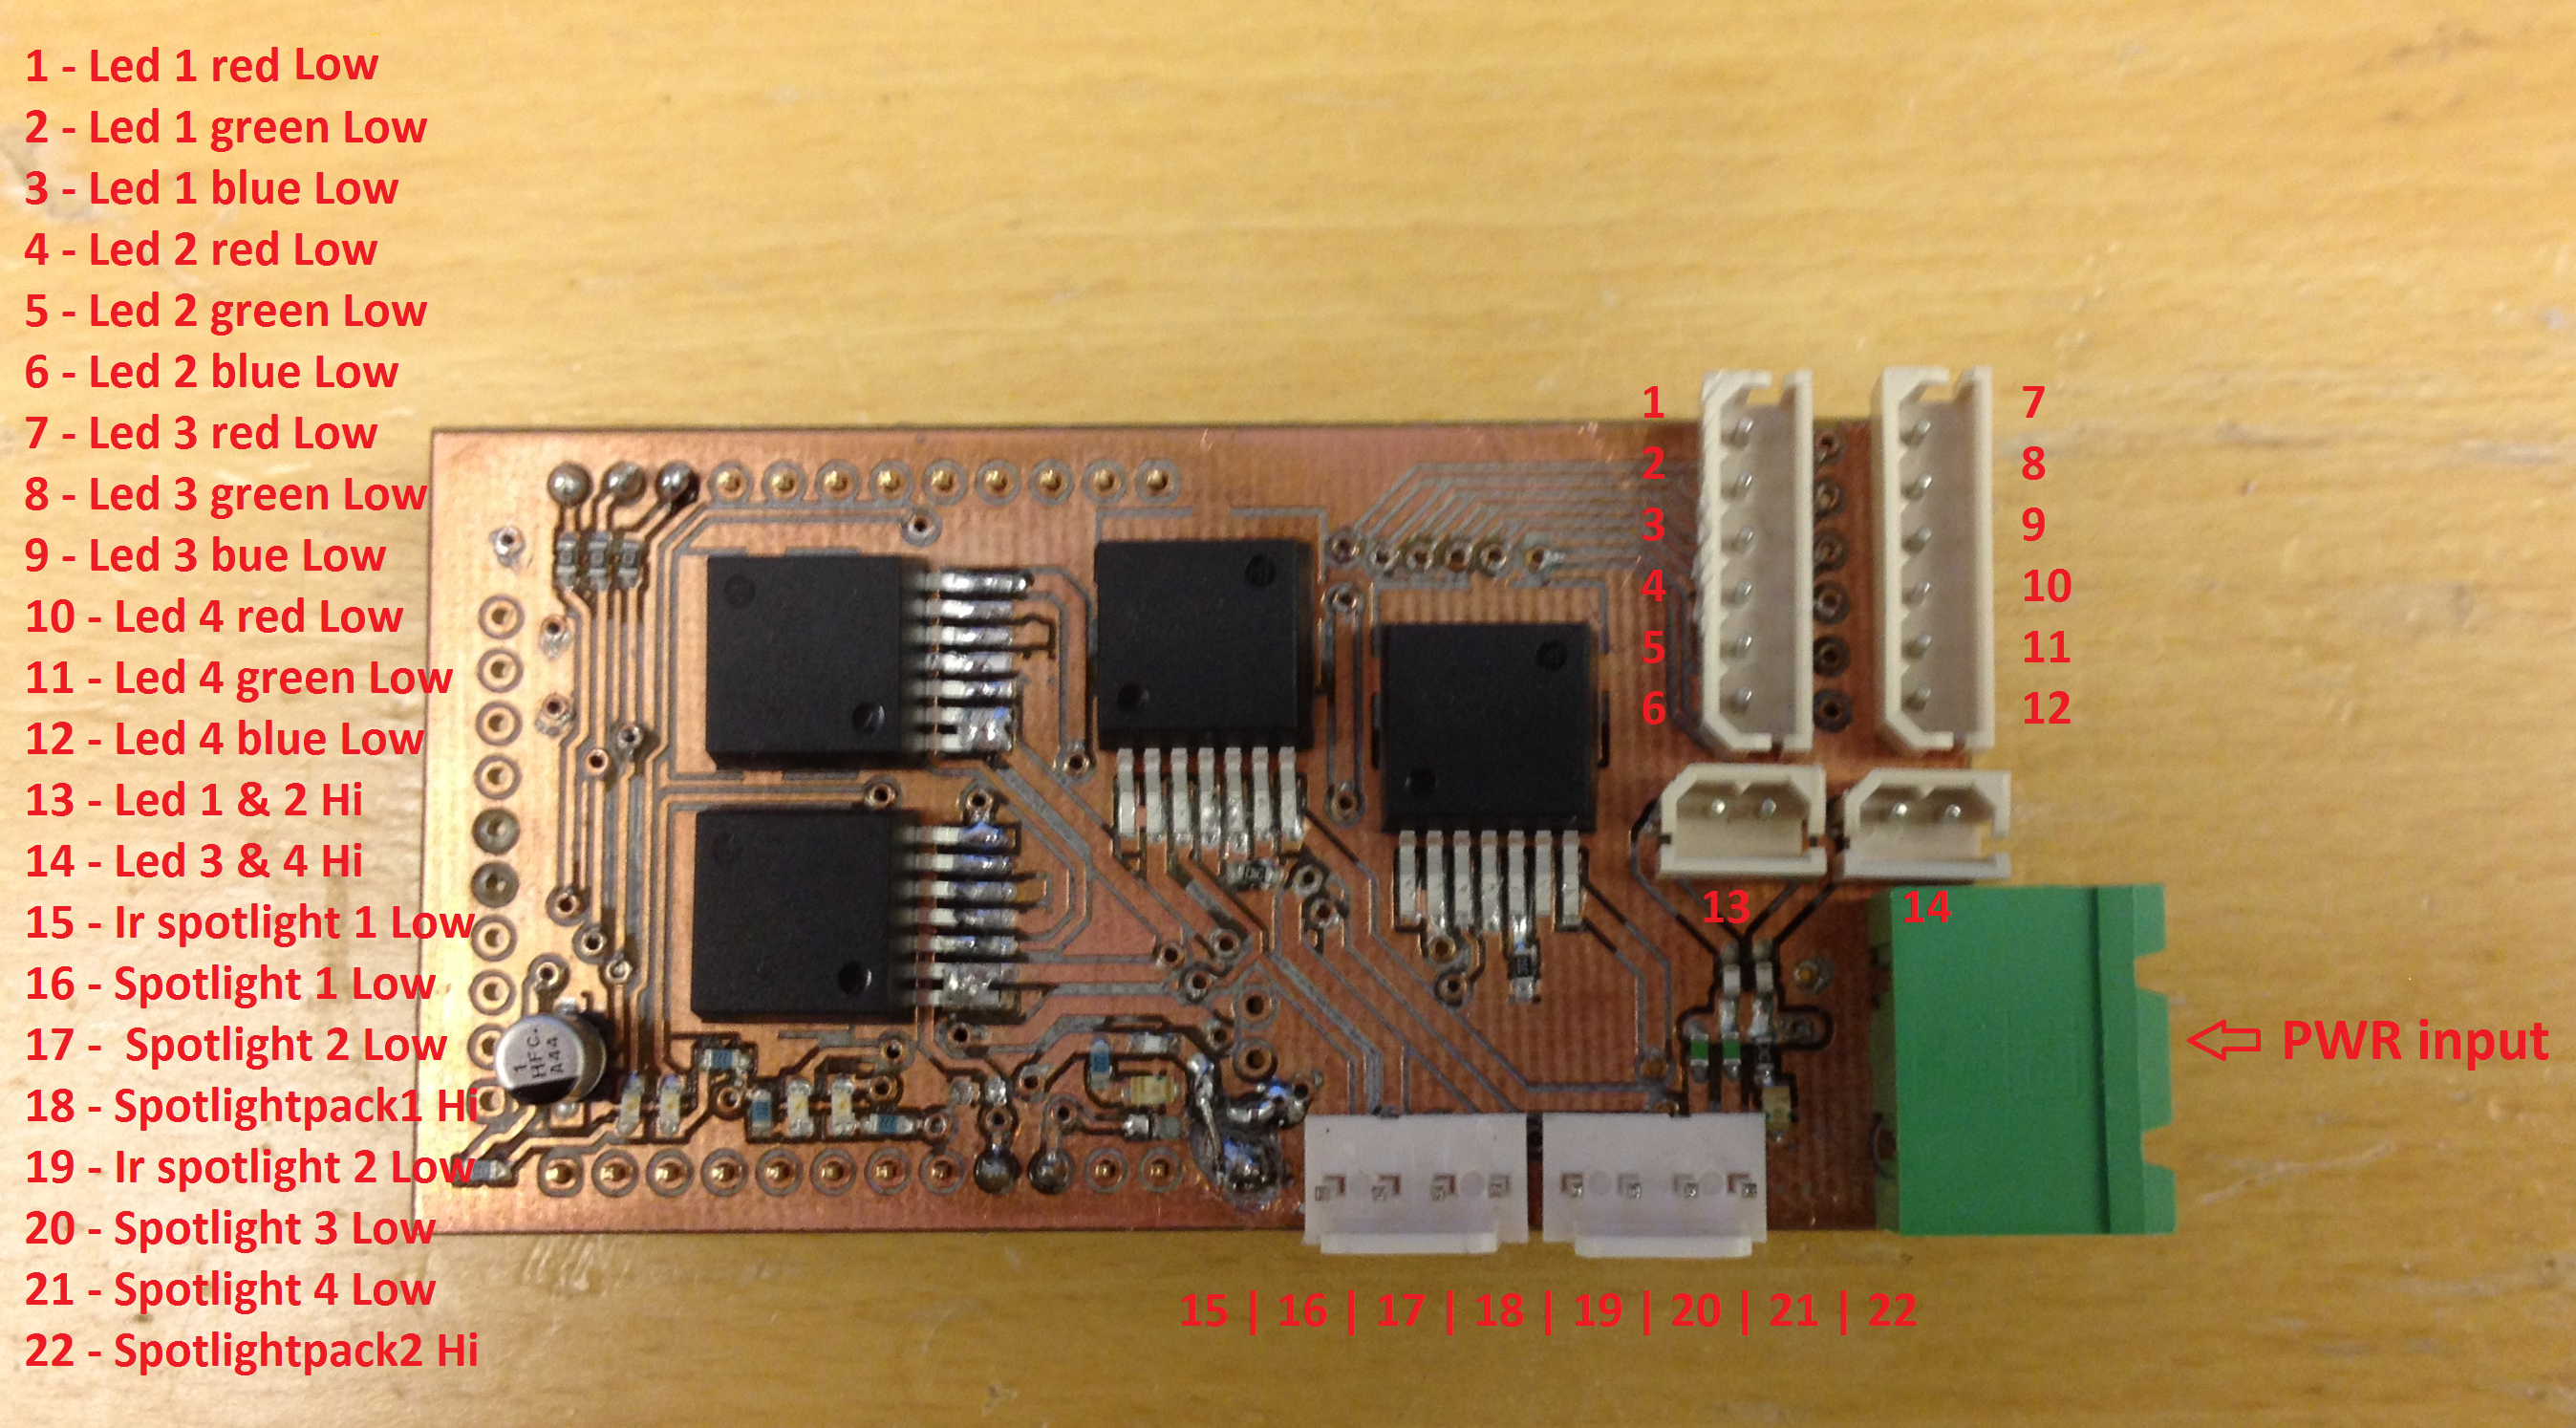
\includegraphics[width=80mm]{./Images/Electronics/LedImgtext.png}
		\caption{Picture of the experimental LED controller board}
		\label{LedImgText}
	\end{center}
\end{figure}

	
 %Written by Lennie

% ============================= Hydrophone =============================
\subsection{Hydrophone} %Patrik
\noindent
One of the missions in the RoboSub competition is to locate the resurfacing point. This location is marked with an acoustic pinger, located at the bottom of the pool underneath the exit site. The pinger sends out a 4 millisecond ultrasonic beep every 2 seconds \cite{robosubrules}. To determine the location of the pinger, four hydrophones are used to determine the direction the sound is coming from. By comparing the differences in time when the hydrophones hears the ping, a direction towards the source can be calculated. The reason for four hydrophones is that, to be able to locate a source in the 3 dimensions, observation of the signal will also be needed in 3 dimensions. With three hydrophones you would be able to get the the angle to the object in the plane, but not know how far off the plane the source is. This setup might have worked in the competition, with the pinger located on the bottom. Since the Naiad is built for a more general purpose, an exact direction in three dimensions is more usable in future applications.

The sound from the pinger needs to be drastically amplified in order for the MCU to handle the signal.The water is not a silent place, so the signal has to be filtered in order to pick up the desired frequency. This is done by the hydrophone shield card, which picks up the signals from the four hydrophones. The card has three main tasks:
\begin{itemize}
\item{Phantom power}
\\The hydrophones gives a much more desirable signal if they are supplied with a constant voltage. This is a done by a voltage division and a big capacitor for stabilization. This power supply can be used for all four hydrophones.
\item{Filter and amplification}
\\The signal runs through a passive high pass filter with a tunable cut off frequency. It is able to filter out frequencies below 10-50 kHz. After the filtering the signal is amplified in two stages. After an  initial amplification the signal is split. One unaltered signal is buffered. Another signal is used as reference voltage for the last amplification stage. These signals are fed as input to the last amplification, where the difference between these two signals are amplified almost 200 000 times to get a clear input to the mcu .
\item{Digitalization and voltage restriction} \\
After the final amplification, the signal is smoothend to a digital high by a capacitor and picked up by one of the interrupt pins on the CAN-card.

\end{itemize}

No equipment for testing the circuit properly has been available. The pinger in the lab is limited to 20kHz and the circuit has worked at close range. No open water test has been conducted. The motors rattle and make a lot of loud noises. Since these sounds origins from a source very close to the hydrophones and the sounds are built from a wide range of frequencies, the sound is almost impossible to filter away, at least with the analog filter approach. Therefor, the only way to pick up the sound from the pinger is to turn the thrusters off and listen, whilst dead in the water.

A digital filter was ruled out due to lack of funds, time and hardware with high enough sampling frequency. The digital filter, with way sharper edges, may have been able to listen for the pings and completely remove any noise from the motors.  	
 %Written by Patrik

% ============================= Speed logger =============================
\subsection{Speed-logger} %Patrik
\noindent
The purpose and mechanical design of the speed logger can be found in section \ref{SL_mec}. The electronics parts of it is divided to an outer sensor and an inner analysing circuit.

\subsubsection{Sensor}
\noindent
The sensor is based on two Allegro A1301 hall sensors. They translates differences in the magnetic field to analogue voltages. These are placed side by side with 5 mm spacing on a small PCB near the rotating turbine. 
The propeller has magnets mounted on its blades, and by reading the timing differences between the sensors, rotational direction and speed can be determined.

\subsubsection{Circuit}
\noindent
The signal from from the sensors needs to be altered in order to work as an interrupt edge for the responsible CAN-card.
The IC circuits on the sensor has a default voltage of half of the supply voltage.
To get an accurate reference voltage, a third A1301 sensor is used inside the hull as a reference voltage.
The difference between the inside and outside sensors is amplified in order to trigger the interrupt on the MCU. 

	
	
 %Written by Patrik

% ============================= Motor extension board =============================
\subsection{Motor configurations}
\subsubsection{Motor extension board} %Anette
The motor extensions board is, in it essence, an adapter. It provides the motor controller with 5V and GND from the CAN card as well as a PWM signal in a suitable connector. It has six three pin WR-WTB connectors from Würth electronics, one for each motor controller. These were chosen since they prevent the user from connecting the cable upside down and is also has a locking mechanism. The current version of the board is made to be used with the 5.0 CAN-card.

\subsubsection{Motor controllers} %Patrik
The controllers was configured with the Castle Link V3.52.10 software. The reason the previous team had trouble with it was that since the firmware was altered from the supplier, some of the files for the setup program had to be replaced. The software is able to configure a number of thruster settings, one of which is the reverse type. The "crawler reverse" setting enables the motors to rapidly change rotational direction in order to make the AUV more agile. %Written by Anette

% ============================= Remote controller =============================
\subsection{Remote control}
When the lid is closed and the Ethernet cable is not plugged in to Naiad there is no easy way to change settings. The remote controller is made to work on land. With the remote control one can navigate and change settings presented on the LCD display. The remote has 4 buttons and one slide switch. The four buttons is for navigating through the menu and the switch is for turning the remote on or off. Since there are no power saving function built in, the batteries in the remote controller will only last for 24 hours unless the switch is turned off after use. The remote uses a commercially bought transmitter and receiver circuit for sending data on the 433MHz FM band. %Written by Lennie

% ============================= Sensor board =============================
\subsection{Actuator board} %Lennie
The actuator board is a board made to control the solenoids for the markers and the torpedoes. The board can have one or two inputs and four outputs. One input can power either two or four actuators depending if the two pins located below the fuses named pwr\_bridge is bridged. The power inputs can be at any level between 0V to 24V. The actuator board does not have any current regulators for the outputs, this is because each output will only be activated for a short time, when the markers get dropped or torpedoes shot. The solenoids that the outputs will power will also be submerged in water, so the heat will not be a problem. Each solenoids is controlled by a digital high/low signal that is sent from a CAN-card. The experimenal actuator board can be seen in fig. \ref{ActuatorImgText}.

\begin{figure}[!ht]
	\begin{center}
		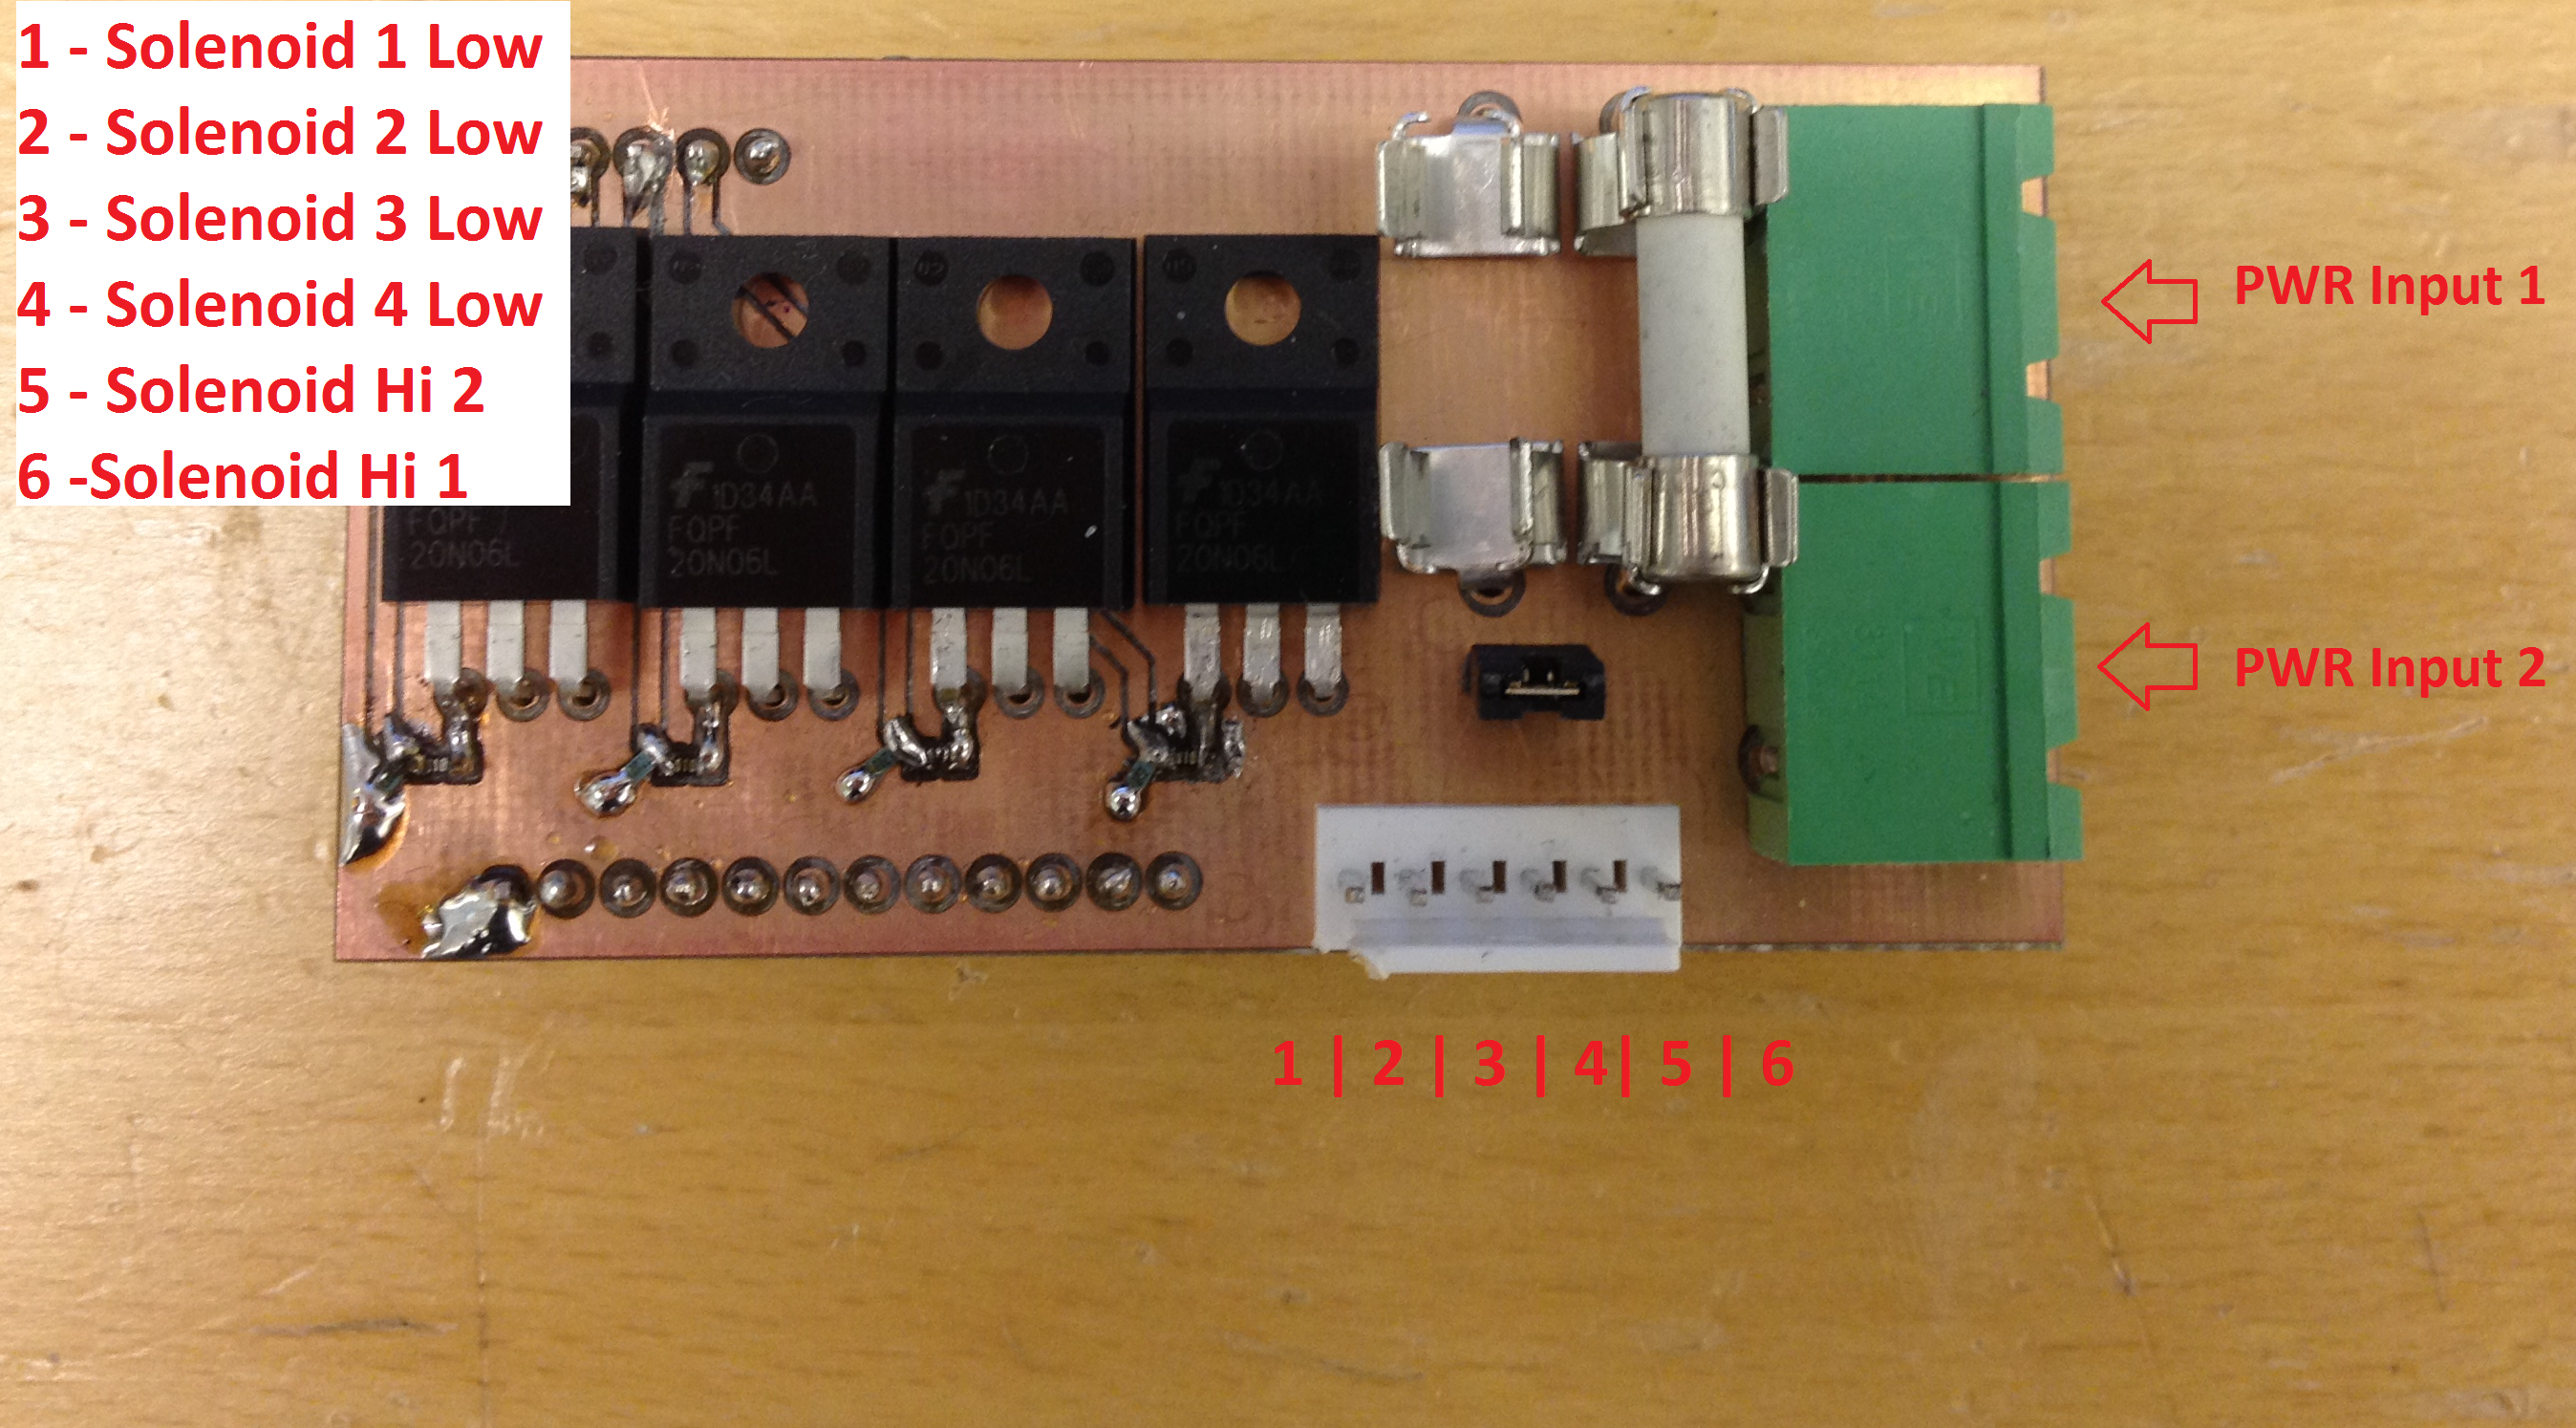
\includegraphics[width=80mm]{./Images/Electronics/ActuatorImgText.png}
		\caption{Picture of the experimental actuator board}
		\label{ActuatorImgText}
	\end{center}
\end{figure}


	
 %Written by Patrik

	
	


% ============================= Software =============================
\newpage%
\section{Software}
% ============================= Introduction =============================
\subsection{Introduction}
\noindent In the beginning the team was split into three subgroups;

The vision group, two persons working full time on vision. Without vision, no missions above regular movement can be achieved, so getting this system to work was crucial for future development.

The Graphical User Interface (GUI) for mission control, one person working for half the project. This part was made so that a person not knowing much or anything at all about the software inside Naiad should be able to program the missions for the competitions or even real missions in the future.

Naiad main control software, three persons working full time and one person working half time. This group had the responsibility to get Naiad moving correctly, in water and simulations, all nodes on the CAN-bus and that all internal and external communication was working as supposed.

The software system is almost redone from scratch, except some firmware and vision from Vasa and old Naiad. The main reason to redo most of the work was to make the complete system more modular, in the end a node based on Transmission control Protocol (TCP) system which is communicating with JavaScript Object Notation (JSON) \cite{JSON} was built. With this system done, the three subgroups (vision, mission interface and Naiad main control) would make it easier to implement and test their software without having to rebuild the whole system. This also lead to a more agile/scrum like development, due to small nodes which could be done and tested faster, without having to change much or anything at all in the existing system.

On the BeagleBone Black (BBB) \cite{BBB} and CAN-bus all code running is written in Ada, the vision is written in C/C++ and external programs are written in Ada, C\#, Matlab and python. 
For the ease of communicating between the same and different languages, the JSON standard was used over TCP. BBB uses  Universal Asynchronous Receiver/Transmitter (UART) to communicating to a CAN-node connected to the CAN-bus that joins everything to one system.

Robustness and reliability are key components in a robot, so most code in Ada has been written taking Ravenscar \cite{Ravenscar} in consideration. Some fail detection is also implemented in the CAN-bus to be able to restart the system if needed. The BBB main routing node can also check what other nodes is connected.

To achieve an greater form of modularity, space plug and play avionics\cite{spnp} have been started to be implemented, as for now when a new CAN-node connects, it will send its name to the power supply unit(PSU) CAN-card, this information will then be passed on to the BBB, this can also be done on request, so that the PSU CAN-card asks the system what cards is still connected, gather the information and send it to the BBB.


\begin{figure}[!ht]
	\begin{center}
		\includegraphics[width=80mm]{./Images/Software/flowchart.png}
		\caption{Complete flowchart of software}
		\label{YourLabel}
	\end{center}
\end{figure}
 %Written by Jonatan

% ============================= Background =============================
\subsection{Background} 
  When the project started this year a lot of the fundamental electronics had already been created. This meant that the overall electronic design was decided as well as thrusters and motor-drivers. The power supply was complete as well as the base of the Controller Area Network (CAN) bus. The Microcontroller unit (MCU) AT90CAN128 was decided as a CAN-bus control unit and stacks to mount and connect the cards was complete. There are a lot of redundancy in the system, for example, each CAN-card transforms from 24 to 5V. An explanation for this from the previous team was to increase robustness in the system. If a leakage occurs and the 5V on the power board and 24V is shortened the CAN-card will not burn. Each CAN-card can handle 12.6-48V making them less sensitive to spikes in the system than if one 5V source would go straight in to all of the MCUs.
  
  	\subsubsection{Generic CAN} %Anette
From the previous team, a generic CAN-card was created that has the version number 4.4. This card has nine analogue and eight digital IO-channels. As well as SPI, two UART channels and CAN-bus interface. The card is equipped with a AT90CAN128 MCU giving each card its own computing power. This makes it possible for the card to interpreted CAN-messages, make computation and give out an response. There was a requirement from last year that all of the sensors were to have its own computing power. This requirement was removed during this project. For the most part the card is fully functional. There are some bugs still though. For example the footprint for the 100nF electrolyte capacitor to the left of the switched DC-DC converter is backwards. This can be seen in fig. \ref{Capacitor}

\begin{figure}[!ht]
	\begin{center}
		\includegraphics[width=90mm]{./images/Electronics/Capasitor.jpg}
		\caption{The capacitor marked C12 have an incorrect footprint, the footprint is backwards compared to the shoe on the capacitor.}
		\label{Capacitor}
	\end{center}
\end{figure}
   
	\subsubsection{Thrusters} %Patrik
\noindent
The previous team had decided to use the Crustcrawler 400HFS thrusters\cite{thrusters}. They are specially designed for AUV and ROV applications, and are, compared to their size, quite powerful. We had no reason to question this decision since they were already mounted and running. The motors were controlled by the Phoenix Ice2 HV 60 motor controller from Castle Creations \cite{motor_drivers}. The drivers, originally designed for RC air crafts, were bought with custom built firmware, designed to be able to instantly switch rotational direction. The previous team had not been able to get the special firmware settings to work.
 
		\subsubsection{Stack}
	To connect and support the CAN-cards a board that makes it possible to stack these on top of each other was created last year. These holders could hold three cards and the cards was soldered to the stacks. This created some problems with fitting add-on cards. Also if a card would break it was difficult to replace unless all three cards was replaced. 
	
	\subsubsection{Power supply unit} %Anette
A power supply unit (PSU) existed, which was created to supply the different parts of the system from a single source. This card have not been changed during this project. A CAN-card on the PSU can control the supply to different parts of the system. The only thing that can not be control entirely by the software on the CAN card is the supply to the motors. For the thrusters to be supplied the they need to be enabled by the card but the kill-switch also need to activated. The kill switch consists of two physical pins than need to be connected in order to supply the motors. This switch can not be overwritten or controlled in software but are built in to the board. The kill switch controls the power to the thrusters as well as the 12V output but \emph{not} the rest of the system. The CAN-bus and 5V output can be started even if these pins are not connected. There are a few patches on the card printed from Würth electronics. These patches has been added to the schematics but no board design has been made. The schematics is backward constructed from the physical card since proper documentation was absent from the previous group. Even though it has been proofed several times there might still be errors it it. To read more on how the card works see appendix \ref{A_powerboard}. The schematics can be found in appendix \ref{Schematics_Power}.

	\subsubsection{Inertial Navigation System board} %Lennie
When the previous group was working on Naiad the design of the Inertial Navigation System (INS) board was started. A design was proposed for the Fiber Optical Gyroscope (FOG) and was built but not tested. During the summer there was another electronics project where one person had as a mission to test the INS board and discovered that it did not work. The design was not working properly, since the circuit was not complete. Instead it worked as an current generator. A new design was proposed during the summer project and a lot of tips for improving the card was proposed. The proposed board was not built so the design ideas could not be tested. During this years project the ideas was taken into account. Improvements was then made and a new card was built and have been undergoing testing.
	 %Written by Jonatan

% ============================= Communication =============================
\subsection{Communication} % Jonatan & Hampus

\noindent All of the node to node communication is based on either CAN or Transmission Control Protocol (TCP) where the former is communication between CAN-cards and the later is between nodes that are either on a BBB, a GIMME-2 card or other nodes that are connected via Ethernet. A node on the CAN-bus is still able to communicate with a node on a BBB by passing through a translation node.

\subsubsection{Node based TCP communication} % Hampus
\noindent All of the TCP communication is routed by a central server node that will relay messages to the desired destination node which is specified in the message itself. Having a central node where all the messages pass through adds a lot of overhead but it also adds a lot of flexibility and simplicity for a user. It allows each client to only require a connection to the server while still being able to communicate with all of the connected nodes. Furthermore, this makes it easy to add more nodes to the system with less effort as the other nodes does not have to establish a new connection, they only have to send a new type of message. The center node can also easier track which nodes are alive and connected rather then track every single cross connection between clients.

\subsubsection{Serial Peripheral Interface} % Hampus
\noindent The SPI on Naiad is using the standard master/slave configuration, where CAN-cards are acting as masters and the attached peripherals are the slaves. There are two peripherals that are using SPI in Naiad, an LCD display and an ADC that is connected to a fiber optic gyroscope\cite{fog}. The highest bit rate possible for SPI on the CAN-cards are 8Mbit per sec as the clock rate of the CAN-card oscillator is 16MHz. The high bit rate is needed as it allows faster data sampling from the fiber optic gyroscope for a better precision when using the data for integration.

\subsubsection{Universal Asynchronous Receiver/Transmitter} % Hampus
\noindent Universal asynchronous receiver/transmitter (UART) is the communication link between CAN and TCP where a CAN-card and a BBB is connected. This link have the lowest communication bit rate which in turn sets the limit of the combined bit rate to and from all of the sensor cards. While the BBB support CAN, it does not support the high voltage that is on the bus which is why UART is used instead. Both the inertial measurement unit (IMU) and the side scan sonar is using UART to send the raw sensor data. The IMU is connected to a CAN-card and the side scan sonar is connected directly to a BBB due to the high amount of raw data it produces. The bit rate for all UART communication is 115200 bits per second.

\subsubsection{Controller Area Network} % Hampus
\noindent The Controller Area Network (CAN) protocol is fully hardware supported on the microcontroller AT90CAN128, supporting the standard CAN controller 2.0A \& 2.0B. Advantages of using CAN is the ease of adding additional nodes and the fact that it is a broadcast protocol. This allows a very modular system where new nodes can enter the bus without the need of establishing connections to already existing nodes. One drawback of CAN is the limited data bandwidth. To reduce the load on the CAN-bus, many calculations are done directly on the CAN-cards, so the data sent is directly usable.
 %Written by Jonatan & Hampus

% ============================= Beagle Bone Black =============================
\input{./Software/Beagle-bone-black} %Written by Jonatan, Joakim and Wenkai

% ============================= GIMME-2 =============================
\subsection{GIMME-2}
The GIMME-2 board system is equipped with two 10 Megapixel image sensors. The GIMME-2 has a zynq processor which has an ARM Cortex A9 dual-core processor and FPGA in the same chip. The board has 8 GB of RAM . There is a slot for external memory storage. The operating system installed on the GIMME-2 board is Peta Linux.  All instructions for  building the operating system on GIMME-2 can be found in appendix \ref{GIMME2}.
	
The system retrieves missions from the decision center and sends back information according to the given mission. Fig. \ref{Gimme_f} explains how the system works. 
\begin{center}
\begin{figure}
\includegraphics[height=10cm]{./Images/GIMME-2/f}
\captionsetup{singlelinecheck=off}
\caption[hej]{\label{Gimme_f}
\begin{itemize}
\item Stereo Cameras: continuously takes images underwater.
\item Image Enhancement: Enhance incoming images from stereo camera.
\item Analyzer: Analyze incoming mission(type of object to detect) and send back required parameters to Mission control center.
\item Object Detection: Detect objects according to the Analyzer and send back feedback to the Analyzer.
\end{itemize}}

\end{figure}
\end{center}

\subsubsection{Operating system}
The operating system used on the GIMME-2 board is Peta Linux 2014.3 customized by Xilinx for Zynq processor which is based on the vanilla kernels. There are two ways the user can interact with the GIMME-2 board either through a serial port interface (USB cable ) or through SSH client(Ethernet cable).
Creating  a bootable Linux for zynq on GIMME-2 board  is challenging due to the fact that the files available on the Xilinx website are mostly for the Zynq evaluation board. The files that are necessary for booting Linux have to be built from scratch, the procedure and tools used for building these files are described in details in Xilinx wiki web site \cite{xilinxuserguide}. 
At first the First Stage Boot Loader (FSBL) starts and does the early system initialization then the universal bootloader starts which loads the kernel image and the wrapped ramdisk image.

\subsubsection{Vision system software}
The software in the vision system is a major issue especially since it is dealing with live captured images in underwater conditions, which have changing lighting conditions that will affect the image detection system.

A vision system has been made using OpenCV to deal with all the issues that the vision system can face. 

In order to have a better calibration between the GIMME-2 cameras and the real live values a red light detection system has been made which was the start for building  the vision system.

\subsubsection{OpenCV for GIMME-2}
OpenCV has been used in order to implement vision methods  since it has a lot of functions that could be used to have a better detection and  enhance the underwater image, the challenge was to build the OpenCV for GIMME-2 board. Arm-linux-gnueabi cross compiler has been used for building OpenCV for GIMME-2. All instructions of building OpenCV for GIMME-2 can be found in appendix \ref{OPENCV}.

\subsubsection{Image Enhancement} 
Underwater images are not clear, when the depth increases, the amount of light on objects decreases and the light distribution becomes irregular \cite{Image_Enhancement}. So before further image processing, enhancement of  incoming images from cameras has been done  by  converting the image to YUV( Y referred to as luminance or luma, while U and V is the chroma) color space and perform Contrast Limited Adaptive Histogram Equalization (CLAHE) on the Luminescence (Y) channel for improving image contrast \cite{Image_Enhancement}. Dilate and erode which are functions used in OpenCV are also used to enhance input images.

\subsubsection{Red Light Detection}
Detecting the red light is very important since that it is the base that all the detection in the vision system depends on especially for the real life calibration. Working with OpenCV, two red light detection systems has been made. The first depends on the red light channels inside the image which called the red boost method \cite{Red_boost_Method}. The second depends on taking the histogram of the red channel inside the picture and back project the most red part in the histogram which is called the histogram method \cite{Histogram_Method}.

The red boost method starts with reading the BGR image and split it into three channels red, green and blue. Then take away the green and blue and  keep the red only. 
Once the green and blue colours is taken away use the multiply function used in OpenCV to boost up the red color only and save the final image in a matrix of type Mat. 
After that, threshold the red boosted using threshold image function used in OpenCV and keep only the highest red and save the threstholded image. The threstholded image will be sent to the moment class used in OpenCV to get the x and y of the center of the detected red.
 
Histogram method works by finding the histogram of the image and then back project the highest red position in the source image. It starts with reading the BGR image and then split it into three planes. Using the split function in OpenCV a green, blue and red plane will be generated and sent into the calcHist function used in OpenCV with a specific histogram range depends on the hue range for the red colour. 

Once the histogram calculation is done for the three planes a normalization is required to assure that the histogram is in the range for the BGR image. Once that is done the highest red can be detected by calling the calcBackProject function in OpenCV \cite{Histogram_Method_in_opencv} which will threshold the image using the hue range  and by that will detect the red light, and this image will be sent to the moment class to get the x and y of the center of the detected red. 

\subsubsection{Object Detection}
For object detection, template matching and shape matching has been tested, but they are not good when the object is rotated or scaled; the irregular light distribution underwater would mean having extensive number of  templates which would be time consuming so feature detection algorithms and classification algorithms has been used to detect the required objects and additional complex objects.

Once the object is detected by the stereo camera, the system will find the necessary parameters. It sends back the x coordinates of the object in both images and then the distance is determined by the difference between these two coordinates.

The distance is found by multiplying F (the focal length of the camera) with B (the distance between the cameras) and divide the answer by disparity (the difference between the x coordinates from left and right images) as seen in equation \ref{equation:1}, and then the final answer is multiplied with a calibrated value to get the distance in real life\cite{Stereo_Camera} \cite{Find_distance}.
\begin{equation}\label{equation:1}
Distance = (F*B)/disparity
\end{equation} 
To find the yaw of the detected object the y coordinates of the detected object is needed and the distance to the object and some gain value found from a lots of testing in real life conditions.
First multiply the difference in x between the object and the center with the distance to the object and the gain value as seen in equation \ref{equation:2}, and then divide the answer by 100 to get the final value in meters as seen in equation \ref{equation:3}.
\begin{equation}\label{equation:2}
pos y= pos y (x difference) * Gain * distance
\end{equation} 
\begin{equation}\label{equation:3}
pos y=pos y/100
\end{equation} 
Finally to find the yaw value of the object the mathematical function arctan is needed with parameters for (pos y) and distance as seen in equation \ref{equation:4}.
\begin{equation}\label{equation:4}
Yaw=atan2 (pos y , distance)*(180/PI)
\end{equation} 
Finding the z position of the detected object  can be done mathematically with the need of distance to the object and some gain value found from a lot of testing in real life condition and finally the y difference between the object and the center as seen in equation \ref{equation:5} and \ref{equation:6} .
\begin{equation}\label{equation:5}
pos z =  pos z  (y difference) *Gain*distance
\end{equation} 
\begin{equation}\label{equation:6}
pos z =  pos z /100.
\end{equation} 

\subsubsection{SURF Algorithm}
 SURF(speeded up robust features)  is a fast, and more accurate algorithm compared to others \cite{SURF_Speed}. When using SURF four steps should be followed:
 \begin{enumerate}
\item Key points selection from both images (object and scene). 
\item Eextraction of descriptors from those key points.
\item Match descriptors by matcher.
\item Analyze  matches \cite{SURF}.
 \end{enumerate}

For matching flann matcher and knn (k-nearest neighbor) matcher has been used, and knn give. Better results. As a final result of SURF it can be a very useful method for complex objects and it can detect some of required objects, but not all of them because they do not have too many features and edges.

The SURF algorithm APIs is not included within the OpenCV repository is intended for development of so called extra modules. All instructions of building extra modules with OpenCV for GIMME-2 can be found in \ref{OPENCV}.

\subsubsection{Classification}
One of the best object detection methods is the Haar Cascade Classifiers. It is a machine learning based method, which uses a cascade trained by hundreds of sample pictures called positive and negative images \cite{Haar_Classification}.

The haar training is the most difficult and time consuming part of the haar cascade method. Once the negative and  positive images is gathered the user can start  making the sample images which combine the negative and the positive images in one file once the samples images is finished the final step left is to start the training and generate the Haar trained file.

The instructions for training your own Haar Cascade can be found in \cite{Haar_Cascade_Training} and
 \cite{Opencv_Haar_Training}.
 
\subsubsection{Gate Detection}
For gate detection the enhanced image has been converted to HSV (Hue, Saturation and Value) and segmented for a specific color. Edge detection is used to separate desired edges, which makes it possible to find contours. %Written by Omar & Nahro

% ============================= CAN-card =============================
\subsection{CAN-card}	%Jonatan & Hampus
\noindent Two versions of the CAN-card is used, the one developed last year and a modified version of that one to be able to use six PWM signals on the same card. 

\begin{figure}[!ht]
	\begin{center}
		\includegraphics[width=80mm]{./Images/Software/gcan_v4_4.JPG}
		\caption{Generic CAN card version 4.4}
		\label{YourLabel}
	\end{center}
\end{figure}

\begin{figure}[!ht]
	\begin{center}
		\includegraphics[width=80mm]{./Images/Software/gcan_v5_0.JPG}
		\caption{Generic CAN card version 5.0}
		\label{YourLabel}
	\end{center}
\end{figure}

To use the analog ports as analog inputs a jumper on AREF is required. For the CAN-bus to work it needs atleast one jumper over CAN Jumper pins in the pictures above, but more is not a problem, so preferably use one jumper on each card.
%label till bilder

The CAN-cards got Atmels microprocessor AT90CAN128 \cite{at90can128} coupled with a 16MHz oscillator. It got hardware support for Serial Peripheral Interface (SPI), Controller Area Network (CAN) and Universal asynchronous receiver/transmitter (UART) protocols. The AT90CAN128 microprocessor is programmed with the JTAGICE MKII\cite{JTAGICEMKII} or JTAGICE 3\cite{JTAGICE3} from Atmel or equivalent together with the software Atmel studio 6.
To program, attach the programmer to the analog pins. 
\subsubsection{Thruster node}
\noindent From the previous years requirement one micro controller should be assigned to each motor. This requirement was removed this year which lead to the decision to let all motors become one node with a mutual micro controller, saving both energy, reducing heat and lessen the load on the CAN-bus.
The PWM signal for the motors runs on 50 Hz and a duty cycle between 5\% and 15\%. The cards receives instructions from CAN messages where a byte of data represents the desired speed.

\subsubsection{Sensor node}
\noindent The sensor node handles all the analog sensors such as the pressure sensor \cite{Pressure_sensor}, the temperature sensor and the salinity sensors. For the time being, only the pressure sensor has been implemented. It is able to give the depth of the unit down to three bars pressure which translates to roughly 20 meters.
A temperature and at least one salinity sensor is planned to be implemented as well in the future to help the system estimate movement etc.
First an sample from the pressure sensor should be taken to measure the value at the surface, the analog-digital-converter (ADC) has a resolution of 10 bits, therefore the resolution of the depth would be 
\begin{equation}\label{first}
20 metres / 2^{10} = 20 000 centimetres / 1024 = cm depth / analog value \approx 2 cm / 1 analog value
\end{equation}


So the real depth of Naiad would be 
\begin{equation}\label{first}
(current value - initial value) * 2 = centimetres below surface
\end{equation}
\subsubsection{Inertial navigation system node}

% Hampus
\noindent The main purpose of the INS card is to get the current orientation of Naiad. This is done thanks to an IMU and a fiber optic gyroscope. The IMU is communicating with UART. The IMU can be configurated to give a variance of data. Currently the outputting orientation in X, Y and Z axis as well as the true body acceleration in X, Y and Z. The output data of the IMU is sent as a string of characters containing both header information and the data itself. The INS card removes all of the header information by extracting specific sections of the string and converting them to float values. This heavily reduces the data that has to be transmitted and it makes the values possible to use immediately. As each float is four bytes and a CAN message can has eight bytes of data, each message can hold two values from the IMU. A total of three messages are required to send all the data for each time the IMU generates an output. The current IMU output frequency is 20Hz. An issue with the IMU is that it can drift in yaw due to the nature of the implementation of the IMU hardware. 

To compensate, a fiber optic gyroscope is added to track the yaw orientation. The fiber optic gyroscope is generating an output voltage correlated to the angular velocity around yaw. This voltage has to be measured very precisely which is why it is connected to an external low noise ADC. The ADC is sending the voltage value via SPI, this allows for a high bit rate which is needed to get a small integration interval. The ADC is acting as a slave in the SPI communication and it requires to first be selected through a slave select pin by pulling the voltage to a digital low. When the ADC is activated, it requires an external clock to drive the transmission. The clock should be starting with a rising edge when transmitting data. The initial procedure of the CAN-card is to send instruction to set the sample frequency of the ADC and also tell it to send data continuously so the CAN-card can avoid asking for data each time. As the ADC uses 24 bits to store the voltage value, each measurement has to be sent over three transmissions as the word size of the SPI is eight bits. The CAN-card will turn the slave off by turning the slave select pin to a digital high. 

\subsubsection{Power supply unit node}
\noindent This node controls how and when to start electronics and motors and also feedback to and from outside the robot in form of an LCD screen and a remote control. By controlling power to other nodes it has the possibility to restart the whole system on command or if needed.
The mission switch is connected to this node, by removing the switch it will send a command to the BBB allowing them to run the mission, if put back during a mission, the mission is paused until the switch is removed.
\subsubsection{Translator node}
\noindent Naiad mainly uses two different communication protocols to communicate between nodes, CAN and TCP. The link between them is UART as the BBB do not support the high voltage of the CAN-bus. The only task for this card is to read all the messages on the CAN-bus and pass them on to a BBB via UART and, vice versa, it translates UART messages to CAN messages. If this card sends too many UART messages over a short amount of time to a BBB, the BBB can crash.  
\subsubsection{LED node}
\noindent When the robot is in the water, debugging and understanding the system by reading the LCD is hard, so by being able to control a total of 4 rows, 2 on each wing, of RGB LEDs, a better understanding is achieved and it will draw more attention to the robot.
The card is also controlling power of the headlights in the front and bottom to support the vision system.
\subsubsection{Hydrophone node}
\noindent As the time difference between the signal generated from the different hydrophones is small, the time stamping for each is based on four different interrupts to avoid busy waiting. When all four interrupts are triggered, a calculation can be made to get the source direction of the sound. The direction calculation is not implemented. When an interrupt is triggered, the interrupt on that pin is disabled. This is required because the CAN-card will get multiple pulses from the same source instance. The interrupt pin is enabled when either all four interrupts have been triggered or after a set time.

%\subsubsection{Speed logger node}
%\noindent 
 %Written by Jonatan & Hampus 

% ============================= User interface =============================
\subsection{User Interface}	
	\subsubsection{Mission control interface design} %Wenkai
	\noindent
The user interface is an integrated development environment, it is a graphical application written in C\#, it allows the user to drag the mission from the missions panel and drop them to the painting panel, use straight line arrow or a curve line arrow to connect the missions. It also includes the PID control setting part and CAN message control part, all the output from this interface are JSON strings.

The flowchart that in fig. \ref{IDE_overall_design} show the whole design of the user interface. First finish the drag-and-drop part, second make use arrow to connect with the node come true, finish the JSON string output through the TCP communication.
\begin{figure}[!ht]
	\begin{center}
		\includegraphics[width=50mm]{./Images/Software/IDE_overall_design.png}
		\caption{IDE over all design flowchart}
		\label{IDE_overall_design}
	\end{center}
\end{figure}

The drag and drop part mainly use the Microsoft Visual Studio tool, the drag part use the toolStrip bar which is a develop tool you can drag button from it easily. The drop part use the painting panel which you can drop some components on it. If there is a task or an arrow was dropped on the panel, then this component is added to the PaintItem List<>. The purpose of doing this is to make sure it is easy to manage all the items on the panel, then the painting panel will trigger the onPaintBackground and onPaint method, so the panel will refresh and repaint. The flowchart that in fig. \ref{drag_drop_design} is the design flowchart for the drag and drop event part.
\begin{figure}[!ht]
	\begin{center}
		\includegraphics[width=80mm]{./Images/Software/drag_drop_design.png}
		\caption{The drag and drop design flowchart of IDE}
		\label{drag_drop_design}
	\end{center}
\end{figure} 
After dropping a task on the panel, the node should still be moveable. When click the mouse, the first thing need to do is to check which side of the mouse was pressed, if it was left button, then set the move value equal to true and get the start position of the node, calculate how far did the mouse move and set the new coordinate equal to the node, refresh the paint panel and set the move value equal to false. The flowchart that in fig. \ref{drag_button_on_panel} is the drag node move on the panel design.
\begin{figure}[!ht]
	\begin{center}
		\includegraphics[width=50mm]{./Images/Software/drag_button_on_panel.png}
		\caption{Drag node move on the panel design of IDE}
		\label{drag_button_on_panel}
	\end{center}
\end{figure}
\subsubsection*{create JSON and subJSON string design}
\noindent
Before trying to create a JSON string, there is one thing that needs to be done, sorting all the items in the PaintItem list<>, add nodes into the unitNameList<>, add straight lines into the straightLineNameList<>. Add curve lines into curveLineNameList<>, and also make sure all the units in order depend on their coordinate by using Sort() method. Until now it is time to create the first JSON object, json1, set the checkMark value equal to false. The checkMark is used to check whether the straight line is the last straight line or not.
 The first thing that needs to be done is to check how many straight lines in the straightLineNameList<>, if there is no straight line, call CreateSubJsonString() function to create a subJSON string which is the callBack string and add this sub string to json1. If there are lines in the straightLineNameList<>, create another JSON object json2, find the last line in the list. Compare the coordinate with all the units in the unitNameList<>, if the unit's coordinate is equal to the line's startPoint, then add the unit name to json2 and also add json2 to json1,set the checkMark equal to true. Now compare all the unit's coordinate with the last line's endPoint and do the same thing as the startPoint, but set checkMark to false. Then use the foreach function to create json string for all the unit that left in the unitNameList<>.
 The flowchart that in fig \ref{Generate_Json_string} is the flowchart design for the create JSON string and subJSON string.
\begin{figure}[!ht]
	\begin{center}
		\includegraphics[width=80mm]{./Images/Software/Generate_Json_string.png}
		\caption{Create json string design of IDE}
		\label{Generate_Json_string}
	\end{center}
\end{figure}
\begin{figure}[!ht]
	\begin{center}
		\includegraphics[width=80mm]{./Images/Software/Generate_SubJson_string.png}
		\caption{Create sub json string design of IDE}
		\label{Generate_SubJson_string}
	\end{center}
\end{figure}

\subsubsection*{PID control design}
\noindent
There are three parts on the PID control panel, the position control part, the orientation control part and the TCP communication part. The user can set the value for P,I,D from position x, position y and position z in the position control. From the orientation part the user can set the PID values for yaw, pitch and roll. When the values are set, the user can type enter the IP address and port number and then send the value to BBB. Since there are a lot of values to be set, there is a save and an import button which will make it easier for the user in not having to input all values every time. 
\subsubsection*{CAN message setting design}
\noindent
In this panel, user can set the ID of the CAN message and also the value of the message, after this the programme can figure out the length of the message and display number on the screen. When the user type into the IP-address and port number and press the send button, the message will be send to Naiad.

In appendix \ref{interface} the different functions of the GUI is described in further detail. 
	\subsubsection{Simulation} %Joakim
	\subsubsection*{Modes}
		\noindent
		The simulation node can be set in two different modes.
		\begin{itemize}
  			\item Simulation mode
  			\item IMU mode
		\end{itemize}
	\subsubsection*{Simulation mode}
		\noindent
		In simulation mode a virtual simulated representation of the Naiad robot is run with simulated sensors and actuators. The simulation allows you to be connected directly to the PID controller through TCP sockets, sending equal data as the real sensor node would have done if the robot was running a real task and receiving the real motor values that the PID controller would send to the real robot. These motor values are turned into estimated forces that is shown as dynamic lines coming from the different motor positions to give a good visualization of the forces that is acting on the robot.
		
		The calculations done in the simulation is based on the physical entities of the robot in order to get as accurate estimations of the forces that are acting on the robot as possible.
		
		By converting the motor values from the PID controller into estimated forces its possible to use these forces in the Newtonian equations to get an estimation of the translation of the robot and motion of inertia equations to estimate the orientation of the robot.
		
		Based on Newtons second law of motion the translational and orientational acceleration can be determined by the equations \ref{sim_pic1} and \ref{sim_pic2}.
		
		\begin{center}
		\begin{figure}[!ht]
		\begin{equation}\label{sim_pic1}
		F=m*a		
		\end{equation}	
		\caption{Base equation to get the linear motion}
		\begin{equation}\label{sim_pic2}
		\tau =I\alpha
		\end{equation}
		\caption{Base equation to get the rotational motion}
		\end{figure}
		\end{center}
		


\begin{center}
\begin{figure}[!ht]
\begin{equation}
\left(
\begin{array}{cccccc}
0.866025 & 0.5 & 0.0 & 0.0 & 0.0 & 0.28\\ 
0.0 & 1.0 & 0.0 & 0.0 & 0.0 & 0.22\\ 
0.866025 & -0.5 & 0.0 & 0.0 & 0.0 & -0.28\\ 
0.0 & 0.0 & 1.0 & 0.355 & 0.230 & 0.0\\ 
0.0 & 0.0 & 1.0 & -0.355 & 0.230 & 0.0\\ 
0.0 & 0.0 & 1.0 & 0.0 & -0.355 & 0.0
\end{array}
\right)
\end{equation}
\caption{\label{ThrusterConfig}Thruster configuration matrix}
\end{figure}
\end{center}

Combined with the Newtonian equations a thruster configuration matrix, found in fig. \ref{ThrusterConfig} was used that is based on the distances and angles of each motor relative to Naiads center of gravity (COG) that makes the motion calculations less computationally heavy and easier to edit.
Each row in the thruster configuration matrix represent the corresponding motors motion components. The first three columns represent the X, Y and Z translational component and the last three columns represents the Roll, Pitch and Yaw rotational components.

\begin{figure}[!ht]
\begin{center}
\includegraphics[width=80mm]{./Images/Software/simforward.png}
\caption{Visual representation of Naiad and forces while running in simulation mode}
\label{simforward}
\end{center}
\end{figure}

To make an accurate estimation of the time varying local coordinate frame that the robot would be in after the forces have acted on the body a rotation matrix is determined by the equations \ref{sim_eq1}-\ref{sim_eq2}\cite{petercorke}.


\begin{figure}[!ht]
\begin{center}
\begin{equation}
R^{'}(t)=S(\omega)R(t)
\label{sim_eq1}
\end{equation}
and,
\begin{equation}
R(t+\delta _{t})\approx \delta _{t}R^{'}+R(t)
\end{equation}
which can be combined to,
\begin{equation}
R(t+\delta _{t})\approx \delta _{t}S(\omega )R(t)+R(t)
\label{sim_eq2}
\end{equation}
\end{center}
\end{figure}

Where S is a skew-symmetric matrix that contains the angular velocities that is integrated from the angular accelerations determined by the Newtonian equations.
		
	\subsubsection*{IMU mode}
In IMU mode the simulator can be set into a passive mode that shows a virtual visual representation of the estimated position and orientation that the system in real time has estimated.
No calculations is needed in this mode more than rotating the virtual robot in the right order. %Written by Joakim & Wenkai


% ============================= Final words ============================
\newpage
\newpage
\section{Results}
The result of this project is a robot that is able to operate, autonomously, under water. The robot has a vision system and a sensor to determine how deep in the water it is. It is also able to execute some basic missions, such as move to a certain position or hitting a buoy.  

The list of requirements as it was given from the client is found in \ref{requirements}. During the time of the project, some items were taken from the list of requirements for different reasons, these are marked with red in the list below.  

\begin{enumerate}
\label{resultlist}
\item Functional requirements
\begin{enumerate}
\item {\color{green}Done: The robot should be built using a mono-hull.}
\item {\color{green}Done: The hull should be easy to open and close.}
\item {\color{green}Done: The cabling should be very efficient and easy to manage.}
\item {\color{green}Done: A communication cable for remote operation should use either Ethernet or an optical fibre.}
\item The robot should be able to operate using external power (preferable through an umbilical including optical fibre/ethernet).
\item The umbilical ends in a box that connects to the robot. 
\item {\color{green}Done: There should be a Kill Switch.}
\item {\color{green}Done: There should be a Mission Switch.}
\item {\color{green}Done: There should be indicators like LEDs and/or LCD-display.}
\item Actuators
\begin{enumerate}
\item {\color{red} Every actuator has its own micro-controller.}
\item {\color{green}Done: All actuators should operate over the CAN-bus.}
\item {\color{green}Done: The motors should preferable be BLDC, but ordinary DC-motors can be used.}
\item {\color{green}Done: Make new own BLDC-driver. One Controller two motors. Remark; this was not done, however the old drivers are now working properly}
\item There should be two droppable markers.
\item There should be two unpowered torpedoes.
\item There should be a simple manipulator that can grip an object and release the object.
\item An LED-light for cameras.
\end{enumerate}
\item Sensors
\begin{enumerate}
\item {\color{green}Done: All low rate sensors should operate over the CAN-bus.}
\item {\color{green}Done: High speed sensors should operate over ethernet (GIMME-2).}
\item {\color{red} Every sensor has its own compute power.}
\item {\color{green}Done: There should be a pressure sensor.}
\item There should be a sensor for water temperature.
\item {\color{red} There should be a sensor for salinity in the water.}
\item There should be a speed logger (measures the speed in two directions.
\item {\color{green}Done: There should be an 9-DOF IMU.}
\item There should be an independent gyroscope for the yaw angle.
\item There should be an active two dimensional sonar.
\item There should be a passive two dimensional broadband sonar (20kHz  - 40kHz).
\item {\color{red} There might be a system for finding direction and distance of cooperative robots based on ultrasonic sensors.}
\item {\color{green}Done: There should be two stereo camera systems or one system that fast and accurate can tilt (Two GIMME-2).}
\item The fibre optical gyro shall be installed.
\end{enumerate}
\item Communication
\begin{enumerate}
\item {\color{green}Done: The communication system between nodes should use the CAN-bus.}
\item {\color{green}Done: The project should study Space Plug and Play Avionics (SPA) system and implement part of it.}
\item {\color{red} There should be a communication mechanism for robot-robot communication (in case of cooperative robots).}
\end{enumerate}
\item Software
\begin{enumerate}
\item The firmware (Software for the micro controllers) should be downloaded via the CAN-bus.
\item The firmware should be handled by a configuration manager.
\item {\color{green}Done: Compare the latest Vasa-code and Naiad-code, extract the best parts. Document the arguments.}
\end{enumerate}
\item {\color{green}Done: There should be a simulator for the mechanical and electronic parts.}
\item {\color{green}Done: There should be a simulator for the software system.}
\begin{enumerate}
\item {\color{red} The simulator should be able to handle more than one instance of the robot.}
\item {\color{red} The simulator should handle inter robot communication.} 
\item {\color{green}Done: The GUI of the simulator should be used to monitor the actual robot in operation.}
\end{enumerate}
\end{enumerate}
\item Missions for Robosub 2014 that shall be implemented.
\begin{enumerate}
\item Pinger: Go and bring things on the bottom and move.
\item Gate: Go through gate with visual servoing. 
\item {\color{green}Done: Bouy: Identify and hit.}
\item Bin: Identify and drop marker.
\item Torpedo: Find opening and fire torpedo.
\end{enumerate}
\item Nonfunctional requirements
\begin{enumerate}
\item {\color{red} The programming language should be Ada and using the Ravenscar profile.}
\item {\color{green}Done: The software should be layered, with hardware support as the first (lowest) layer.} 
\item {\color{green}Done: The software should be based on principles for component based software engineering.} 
\item {\color{green}Done: The documentation should be written using Latex.}
\item {\color{green}Done: The preferred computer in the system is the GIMME-2.}
\item {\color{green}Done: The batteries should be easy to change.}
\item {\color{green}Done: Make a complete test plan.}
\end{enumerate}
\end{enumerate}

Most of the items not listed as done are at least started, many of them are almost finished but had to be left that way due to lack of time and\slash or funds. The different items marked in red were removed for different reasons. The requirement that every sensor should have its own compute power was removed, since that would require an extensive amount of extra cards inside Naiad. This takes up additional space and also creates heat inside the hull. All requirements that were related to inter robot communication were removed in agreement with the client since creating more than one instance of Naiad would not be possible during the time of the project. Furthermore, the requirement for writing all code in Ada was removed since it was not possible to run Ada on the GIMME-2 board. The vision programming was done in C instead. However, Ada has been used for all on-robot communication except on the GIMME-2 boards. Ravenscar was also taken in consideration when this was possible. 
\subsection{Mechanics results}
The previous group had developed and constructed the main hull. Since the main hull was complete it was mostly peripherals that needed to be created this year. For example the wings. The wings has been 3D-printed with attachments, such as LEDs to show state in the program as well as mountings hydrophones. 

Also the entire tool plate needed to be redesigned. The tool plate was divided in to a front and back tool plate and are designed to be changeable in case other functionality was desired. The front tool plate has been constructed, it contains most of the equipment for the RoboSub competition. For example torpedoes and markers. The side scan sonar is also mounted in the front tool-plate. The back is at the moment an empty support structure where tools can be attached. The simple manipulator has not been finalised since the project ran out of time. 

\subsection{Electronics results}
The electronics group has continued the work from the previous year and added more functionality to the pre-existing cards. This added functionality have for the most part been by add-on cards to the exiting cards. A redesign of the CAN-card has also been done in order to get more out of the MCU itself. This new card can not at present time completely replace the cards developed last year but it is the belief of the group that this can be done with another redesign.  

Some of the functionalities that has been added is hydrophones to be able to hear a pinger used in the RoboSub competition. A speed logger to help determine the position in the water. The previous group worked on a card to support the FOG to help determine yaw position that this group seems finalised but more testing is required. RGB-LEDs have been added to the wings to communicate with the surface. A remote control to navigate through menus on the display when Naiad is on the surface has been constructed as well as a card to control the solenoids in the tool plate, these have also not been tested however. Also a side scan sonar has been built in to in to the system.  

\subsection{Software results}
Most of the software and protocols running in Naiad have been tested extensively. By observation over time or by trying to break them. If an essential program failed, it has been prioritized until working as desired. By focusing on robustness, a good base for future work has been built.

A lot of work has been put in to get a node based system running. With that working much time can be saved for testing new sub-programs since it is easy to add a new node. It also simplifies diagnostics to see what node is alive to take appropriate actions if a node goes down. This also helps for testing the robustness of that program. 

The PID-controller and path-planner have been tested both in simulation and in real life. The tests have been successful but some tuning is sting required to get optimal performance.

The simulator has been tested with orientation and translation with correct results.
The graphical user interface is yet to be implemented for sending missions to the robot. Tests for sending simulated missions and messages has been done successfully. Implementation in Naiad for receiving missions and messages from the GUI is not implemented.

The vision system has been tested with acceptable result for the purpose, a problem have been the lenses narrow visual angle causing it to easy loose sight of objects. Also the frequency of the program needs to be increased to work efficient enough.

Most of the CAN-nodes works without any problems. The most common problems seems to be caused by SPI or UART, the time needed to firmly fix the firmware for these protocols has not been prioritized due to time issues and that the impact would not be essential.

\newpage
\section{Discussion}
\noindent
The documentation of the work previously done in this project was not that well done, some parts were missing and some parts had faults in them. This made it harder for the team to move forward in their efforts to finish the project. Since the project was already started, the team members agreed that the best way was to continue with what already started. Restarting would have taken too much time. However as the project progressed, it was clear that some parts were to undocumented, others did not reach the right standard and had to be dismissed for that reason. This is to be seen as one of the main reasons as to why the project could not be finished on time. Not all parts had to be redone, some was harder to change, such as the hull which would have taken a lot of money and a lot of time to redo. Some parts were also fully functioning, which made it unnecessary to change them. 

The reason why the umbilical cord was never implemented was that a sponsor withdrew at the last minute and since the cord was too expencive to buy, it was put on hold. However, with the added functionality of the remote, the need for an umbilical cord which is easy to connect and disconnect is reduced, since some of the communication which should have been done through this is instead done via the remote control. An advantage of actually having an umbilical cord would have been the possibility to run Naiad on external power rather than batteries. 

Since the system is currently specified for some of the RoboSub 2014 missions, this will have to be changed before the competition. However, there are only minor changes to the missions which means this will be an easy task. 

Working in a larger group with shared documents have caused problems. Almost all documents was accidentally erased twice, only being able to be retrieved thanks to a computer not updated the folder. Working as a group there is also a possibility that more then one person is working in the same document at the same time. If saved by one this will overwrite the others. This have happened way more than once. For these reasons a better system then Dropbox should be used for sharing files.

The previous Naiad team had one person who was working full time on marketing and getting sponsors for the project. Since there was only 12 persons in this project group, it was decided that there was to many other things to do. This responsibility was supposed to be shared between all members of the group. However in the end, it was only the project manager working on this. As the project progressed it was apparent that the project would have benefited from having one person working full time on this since dedicated efforts are needed to get companies to move forward with sponsoring requests. 

\subsection{Mechanics discussion}
\noindent
The mechanics group is the group that have had to mostly adapt to what was given. This has both been a blessing and a curse. Some decisions on design was already complete meaning some workaround was necessary. At the same time a as it has been good to have a base to start from. Because of time and cost in manufacturing all of the constructed pieces from last year had to be kept. For the most part the designers from last year hat thought abut how to attach the missing pieces. One place where this was not taken in to account was the wings. There are no way to attach the wings into the top of naiad at the beginning. Also the thrusters needs to be graced aver every-time they have been in water. Meaning access to them is necessary. This complicated the design of the wings.

The tool-plate is milled just like the rest of the hull. Milling however eats allot of time. It is hard to get time on the milling machine in Eskilstuna. Every time someone else had used the machine it needs to be recalibrated which also ate a lot of time. To reduce the amount of people wanting time on the machine as well as the complexity on some parts drove the mechanics group to learn the biggest milling machine available in Eskilstuna. This machine has a steeper learning curve than the other machines. Despite the extra time to learn it the conclusion is that is was the right choice. 

The wings and some other smaller parts of the parts produced this year was printed in the schools new 3D-printer. This have not always been without frustration. It is not a high quality printer and sometimes several prints needed to be made before a satisfactory print was done. The printer material also did not seam to go with the chlorine in the pool we were testing the robot in. It is believed that a layer of paint will fix this. 

Another frustration for the mechanics group is the vague description or waiting in response on how things should be mounted by other groups. This is something that is always a problem in all group assignment but because we only had one shot on most of the mechanic pieces it was extra important to get it all right the first time. 

\subsection{Electronics discussion}
\noindent
The electronics groups progress went really smoothly in the beginning. The cards from last year was already produced and add-ons seamed easy. However as the project progressed, the more important it was, to not only be able to use the cards from last year, but also understand them. Most of the documents regarding electronics from last year was sub-standard or missing completely therefore work on recreating this documentation have been done as well, taking up surprisingly large amount of time.

The electronics group have produced allot but as always when constructing hardware it takes longer time than expected and there had been an hope to reach further that we have done. For example have time to order final version cards from Würth and ideally even have time to produce these cards. This have not been the case. All cards have been prototyped and tested but further works needs to be done on most cards. 

\subsection{Software discussion}
\noindent
The software group has worked well together reaching most of the primary goals, achieving a reliable base for future work.

Documentation is just as important as the work you document on in projects of this magnitude. The documentation from the first Naiad team was hard to follow, this led to that almost all of their work had to be redone.
This year the software team has focused on following a standard that should be easy to use and using at most 3-5 layers of code in libraries to avoid having to spend much time understanding where values and functions descend from.

By combining the previous firmware from Naiad and from Vasa, a well working firmware has been achieved in short time, there is still some issues, but overall it works good.

From the start the GIMME-2 boards was supposed to replace BBB but due to limitations of the operative system running on the GIMME-2 boards this would not be an effective alternative.

A lot of problems hard to explain have occurred in the CAN-cards. Whether it is Ada or the firmware that causes it, the persons working with have tried to figure out but without any real success. This are not logical issues, but rather for example crashing when leaving a procedure, variables changing values without reasons etc.

\newpage

%\section{Acknowledgments}

% ============================= References ============================
\newpage
\bibliographystyle{plain}
\bibliography{./Bibliography/NAIAD}
\addcontentsline{toc}{section}{References}

% ============================ Appendices =============================
\newpage
\begin{appendices}

	\section{Electronic schematics}
% Powerboard
%\subsection{Powerboard}
\label{Schematics_Power}
\begin{figure}[!ht]
	\begin{center}
		\includegraphics[width=13.2cm]{./Images/Powerboard_Scematics/Toplevel.jpg}
		\caption{Topview of Powerboard}
	\end{center}
\end{figure}

\begin{figure}[!ht]
	\begin{center}
		\includegraphics[width=13.2cm]{./Images/Powerboard_Scematics/Saftey_supply.jpg}
		\caption{Saftey for supply on Powerboard}
	\end{center}
\end{figure}

\begin{figure}[!ht]
	\begin{center}
		\includegraphics[width=13.2cm]{./Images/Powerboard_Scematics/Saftey_CAN.jpg}
		\caption{Saftey for CAN bus for Powerboard}
	\end{center}
\end{figure}

\begin{figure}[!ht]
	\begin{center}
		\includegraphics[width=13.2cm]{./Images/Powerboard_Scematics/Switching.jpg}
		\caption{Control what supply to use and kill switch Powerboard}
	\end{center}
\end{figure}

\begin{figure}[!ht]
	\begin{center}
		\includegraphics[width=13.2cm]{./Images/Powerboard_Scematics/Current_monitor.jpg}
		\caption{Current sensor to detect how much power the system use}
	\end{center}
\end{figure}

\begin{figure}[!ht]
	\begin{center}
		\includegraphics[width=13.2cm]{./Images/Powerboard_Scematics/5_const.jpg}
		\caption{DC-DC for the constant 5V trace on Powerboard}
	\end{center}
\end{figure}

\begin{figure}[!ht]
	\begin{center}
		\includegraphics[width=13.2cm]{./Images/Powerboard_Scematics/5_out.jpg}
		\caption{DC-DC for the 5V output on Powerboard}
	\end{center}
\end{figure}

\begin{figure}[!ht]
	\begin{center}
		\includegraphics[width=13.2cm]{./Images/Powerboard_Scematics/12V.jpg}
		\caption{DC-DC for the 12V output on Powerboard}
	\end{center}
\end{figure}

\begin{figure}[!ht]
	\begin{center}
		\includegraphics[width=13.2cm]{./Images/Powerboard_Scematics/Variable.jpg}
		\caption{DC-DC for the variable output on Powerboard}
	\end{center}
\end{figure}

\begin{figure}[!ht]
	\begin{center}
		\includegraphics[width=13.2cm]{./Images/Powerboard_Scematics/monitor.jpg}
		\caption{Voltage and temperature monitor for Powerboard}
	\end{center}
\end{figure}

\begin{figure}[!ht]
	\begin{center}
		\includegraphics[width=13.2cm]{./Images/Powerboard_Scematics/MCU_CAN.jpg}
		\caption{Connection with MCU CAN card on Powerboard}
	\end{center}
\end{figure}

\begin{figure}[!ht]
	\begin{center}
		\includegraphics[width=13.2cm]{./Images/Powerboard_Scematics/Outputs.jpg}
		\caption{Outputs on Powerboard}
	\end{center}
\end{figure}

%\subsection{CAN 4.4}

\begin{figure}[!ht]
	\begin{center}
		\includegraphics[width=13.2cm]{./Images/Powerboard_Scematics/Can_4.4.jpg}
		\caption{Generic CAN-card 4.4}
	\end{center}
\end{figure}


%\subsection{Speedlogger sensor}

%\subsection{Speedlogger Control}

\begin{figure}[!ht]
	\begin{center}
		\includegraphics[width=\textwidth]{./Images/Powerboard_Scematics/SL_Shield_v1.2.png}
		\caption{Speedlogger sensor card}
	\end{center}
\end{figure}

%\subsection{INS-board} 

\begin{figure}[!ht]
	\begin{center}
		\includegraphics[width=\textwidth]{./Images/Powerboard_Scematics/INS_schematics.png}
		\caption{Speedlogger sensor card}
	\end{center}
\end{figure}

%\subsection{Sensor shield} 

%\subsection{LED shield}
 \begin{figure}[!ht]
	\begin{center}
		\includegraphics[width=\textwidth]{./Images/Powerboard_Scematics/LED_schematics.png}
		\caption{LEDcontrol-board}
	\end{center}
\end{figure}

%\subsection{Speedlogger} 
	\clearpage
	
	\section{System test}
\section*{Introduction}
\noindent
The goal for the tests described in this test plan is to get the Naiad robot ready for competing in RoboSub 2015 in San Diego, USA. In order to easier find the problem if one should occur, some tests to find the problem has been constructed. 
These tests can be looked at as sort of a flow chart of what to do if something is not working as it is supposed to. Please note that no software will be tested in these tests. 

\subsection{The vision system is not working properly}
\subsubsection*{Purpouse of the test case}
The purpouse of this test case is to find the problem when the GIMME-2 board is not working properly. 
\subsubsection*{Description}
There are a number of different problems that can occur when using the GIMME-2 in Naiad. This test is designed so that finding the problem should be easier.
\subsubsection*{Resources}
Electronics of Naiad including at least one GIMME-2 board with lenses on the camera sensors and a multi-meter. 
\subsubsection*{Preconditions}
Before starting this test the electronics should be powered up and the system should try taking and analysing pictures from the GIMME-2, however for this test to be relevant there has to be a problem somewhere in this process. 
\subsubsection*{Post conditions}
The goal for this test is that the GIMME-2-system should be working properly. 
\subsubsection*{Flow of events}
First thing to check is that the GIMME-2 is powered correctly. Check this using a multi-meter, there should be 12 V where the GIMME-2 is powered see fig. \ref{GimmePower}. 
\begin{figure}[!ht]
	\begin{center}
		\includegraphics[width=80mm]{./Images/Tests/Gimme-power.jpg}
		\caption{Measure on the black and red dot, there should be 12 V between them.}
		\label{GimmePower}
	\end{center}
\end{figure}
If there is no power to the GIMME-2 card, make sure to check the connections back to the batteries from the GIMME-2. Make sure to check the cables and the power board for the GIMME-2. Important to remember when checking this power board is that the card is inverted so that the plane is Vcc and that the trace is ground. The input to this board should 24 V and the output 12 V. 

If all of these seem to be correct, the problem is probably with the GIMME-2 board, this is not easy to fix, replace the card. If the card seems to be working but the vision system still is not, the problem might be in the software for the vision system. 

\begin{tabular}{| l | c |}
\hline
Check point & Measured \\ \hline
Measure power input in GIMME-2 & \\ \hline
Check cables & \\ \hline
GIMME-2 power board & \\ \hline
\end{tabular} 

\subsubsection*{Inclusion/Exclusion points}
This test counts as a pass if the problem can be found and the GIMME-2 board starts working. All other results will count as fails. 
\subsubsection*{Special requirements}
There are no parameters for this category. 

\subsection{Markers are not releasing as they are supposed to}
\subsubsection*{Purpouse of the test case}
The markers might not release as they are supposed to, the purpouse of this test is to find out why this problem occurs. 
\subsubsection*{Description}
This test is designed to find the reason to why the markers are not releasing properly. 
\subsubsection*{Resources}
Complete system including electronics and mechanics.  
\subsubsection*{Preconditions}
For this test case to be relevant the markers should not be releasing as they are supposed to. 
\subsubsection*{Post conditions}
The markers release when supposed to. 
\subsubsection*{Flow of events}
The first thing to check is that the markers are free to release. The next thing to check is to make sure that the solenoid is connected properly. Make sure to also check that the actuator shield is connected properly to its CAN card and that the CAN card is connected properly to the stack. After doing all of these things the next thing is to make a complete unit test of the actuator shield, and if that does not work a unit test on the CAN card should be done.

\begin{tabular}{| l | c |}
\hline
Check point & Measured \\ \hline
Marker can release properly &  \\ \hline
Solenoid connection &  \\ \hline
Actuator shield connection &  \\ \hline
CAN connection & \\ \hline
Actuator shield unit test & \\ \hline
CAN card unit test & \\ \hline
\end{tabular} 
\subsubsection*{Inclusion/Exclusion points}
There are no exclusion points to this test. 
\subsubsection*{Special requirements}
There are no special requirements for this test. 

\subsection{A sensor is giving out a faulty value}
\subsubsection*{Purpouse of the test case}
There are a number of sensors on the Naiad system, the purpouse of this test is to identify the problem when one of them is giving out a faulty value. 
\subsubsection*{Description}
It might happen that one of the sensors give out a fault value, which could make the AUV act inappropriately. This test is designed to ensure how to find the problem if that were to happen. 
\subsubsection*{Resources}
Electronics of Naiad including the affected sensor(s).
\subsubsection*{Preconditions}
A sensor in the system is giving out a faulty value when reading it in software. 
\subsubsection*{Post conditions}
The desired post condition is that the sensor works properly. 
\subsubsection*{Flow of events}
The thing to start with is checking that the sensor is connected properly, that the sensor shield it is attached to is mounted on its CAN-card properly and that the CAN-card is properly connected to its stack. If all of this is properly connected and the sensor is still giving out a faulty value, turn to the respective unit test of that sensor or the card it is mounted to. If the problem is still not resolved, make sure to do a complete unit test on the CAN card the sensor is connected to. The unit test for the CAN cards can be found in appendix \ref{CAN_unit}.

\begin{tabular}{| l | c |}
\hline
Check point & Measured \\ \hline
Sensor connection &  \\ \hline
Shield connection &  \\ \hline
CAN connection & \\ \hline
Sensor shield unit test & \\ \hline
CAN card unit test & \\ \hline
\end{tabular}   
\subsubsection*{Inclusion/Exclusion points}
This test does not test the sensors, it is just testing the connections and the mountings. 
\subsubsection*{Special requirements}
No special requirements for this test. 

\subsection{System does not start}
\label{nostart}
\subsubsection*{Purpouse of the test case}
The purpouse of this test is to find out what is wrong if the system will not start when you power it up. 
\subsubsection*{Description}
This test was created to ease problems with a system that does not start as it is supposed to. 
\subsubsection*{Resources}
Complete Naiad with electronics, batteries and hull, a multimeter,
\subsubsection*{Preconditions}
The robot is not starting when the batteries are plugged in. 
\subsubsection*{Post conditions}
For passing this test, the system should start after this test. 
\subsubsection*{Flow of events}
Start by checking the connection from the batteries to the power cords. It they are connected continue with checking the power level on the batteries. This can be done using a multimeter. The batteries should measure above 22 V, if using a battery monitor all cells should be indicating green. If the voltage is running low, try charging the batteries and then start up the system. If the charger will not charge a battery that could mean that a cell is damaged, discard the battery. 

The next step is to check the Power Supply Unit (PSU), the first thing to look for is the fuse on the PSU. This is marked in fig. \ref{PSU_fuse}
\begin{figure}[!ht]
	\begin{center}
		\includegraphics[width=80mm]{./Images/Tests/powerboard_fuse.jpg}
		\caption{The red square indicates where the fuse can be found on the PSU}
		\label{PSU_fuse}
	\end{center}
\end{figure}
If the fuse is broken, make sure to replace it with a new one. Test if the system will start again. If this did not work, make a complete unit test of the PSU. The complete unit test of the PSU can be found in appendix \ref{Unit_PSU}.

\begin{tabular}{| l | c |}
\hline
Check point & Measured \\ \hline
Battery connection &  \\ \hline
Power level batteries &  \\ \hline
Fuse status & \\ \hline
PSU unit test & \\ \hline
\end{tabular} 
\subsubsection*{Inclusion/Exclusion points}
This test will be counted as a pass if the system starts, all other results will count as fails. 
\subsubsection*{Special requirements}
There are no special requirements for this test. 

\subsection{Is the hull water tight}
\subsubsection*{Purpouse of the test case}
The purpouse of this test is to make sure that the hull is waterproof and that it will not leak when put in water. 
\subsubsection*{Description}
This test is to be performed when something has been added or removed which affects the openings of the main hull. For a description of how to prep the hull for under water usage, check appendix \ref{hullmanual}.
\subsubsection*{Resources}
Required resources for this test is the hull of Naiad, some paper, petroleum jelly, a long rope, and weights (for example in a weight belt for diving). A pool to sink the hull in is also required. 
\subsubsection*{Preconditions}
The preconditions for this test is to fill the inside of the hull with toiletpaper to easier see if there is any intake of water. The hull should then be closed according to the specification found in appendix \ref{hullmanual}.
\subsubsection*{Post conditions}
The post conditions are the same as the preconditions. 
\subsubsection*{Flow of events}
Enough weights to sink the hull should be attached to the hull, make sure that the weights can not fall of when the hull moves around. It should be sunk to the bottom of the water and then left there for at least five minutes. Then it could be lifted from the water and dried on the outside. The lid should then be opened and the inside examined to see that there is no water on the inside. 

\begin{tabular}{| l | c |}
\hline
Check point & Measured \\ \hline
Closed properly &  \\ \hline
Weights attatched &  \\ \hline
Sunk & \\ \hline
Lifted & \\ \hline
Outside dried & \\ \hline
Inside dry & \\ \hline
\end{tabular}
\subsubsection*{Inclusion/Exclusion points}
The depth to which the hull is waterproof is not tested in this test. 
\subsubsection*{Special requirements}
There are no special requirements for this test. 

\subsection{Motor not starting}
This case is a common problem in which one or more motor(s) for some reason is not starting.
\subsubsection*{Purpouse of the test}
The purpose of this test is to identify the problem with the motor and find out why the motor is not running. 
\subsubsection*{Description}
The test is designed to identify any problems with why a motor is not running. 
\subsubsection*{Resources}
One person is required to perform the test. 
\subsubsection*{Preconditions}
The motor is not running on command.
\subsubsection*{Post conditions}
The desired post condition of this test is a motor that is running. 
\subsubsection*{Flow of events}
When the motor is not working that means one of two things. Either the motor is completely quiet or the motor gives out a 2Hz beep-signal. 

If the motor(s) is completely quiet that would imply that there is no power to the motor. In that case all the cables to the power supply needs to be checked. These cables are thick, one is red and the other one is black, and will come from the motor controller and should be plugged in to the PSU. Also the cables to the motors need checking, that is three cables, they are red, white and black from the motor controller and should match the shrink tubing on the cables going out to the motors. When checking the cables - make sure that the conwtb-female has not started to be loose, in this case the contact needs to be switched to a new one. 

If the motor(s) are giving out a beeping signal at 2Hz, that would mean that there is no signal to the motor(s). In this case the signal cable need checking. This cable is orange/red/black and run from the motor controller to the motor extension board. Make sure that the motor extension board is properly connected to the CAN-card. Also make sure that the CAN-card is properly connected to the stack.  

If all the cables and cards are plugged in as they are supposed and the system is still quiet this could mean that there is no power in the system, in this case, nothing should be working and all LEDs should be turned off. In this case, check that the batteries are plugged in and that they are charged properly. How to do this is better specified under \ref{nostart}.

If there is power in the system even if the motor is silent and all the cables are connected correctly then this would mean that the PSU is not working properly. To test this card, use the complete unit test for the PSU found in appendix \ref{Unit_PSU}.

\begin{tabular}{| l | c |}
\hline
Check point & Measured \\ \hline
2Hz beeps &  \\ \hline
Power cables to motor controller &  \\ \hline
Cables from motor controller & \\ \hline
conwtb-female & \\ \hline
Signal cable to motor controller & \\ \hline
Motor extension board & \\ \hline
CAN-card connection & \\ \hline
System power & \\ \hline
PSU unit test & \\ \hline
\end{tabular}
\subsubsection*{Inclusion/Exclusion points}
This test does not test wether the motor is working or not. If the test is failed one could further test this.  
\subsubsection*{Special requirements}
There are no special requirements. 
	\clearpage
	
	%\section{Mechanic tests}
Following is a series of tests that should be performed on the mechanical parts of the system. 

\subsection{Testing the o-ring}
\label{oring}
\subsubsection*{Purpouse of the test case}
The purpouse of this test is to make sure that there are no dents in the o-ring, which would make it unsafe to use under water. 
\subsubsection*{Description}
For this test a person will feel through the o-ring to make sure that there are no dents in it. 
\subsubsection*{Resources}
O-ring, petroleum jelly
\subsubsection*{Preconditions}
The preconditions are that the o-ring is dry and grease free. 
\subsubsection*{Post conditions}
After preforming this test the o-ring should be greased and for a pass it should have no dents. Any dents will count as a fail in this test. 
\subsubsection*{Flow of events}
For this test the person performing the test should have some petroleum jelly on their fingers and gently feel every piece of the o-ring to make sure that there are no dents in it. Make sure that the entire o-ring is properly greased. 

\begin{tabular}{| l | c |}
\hline
Check point & Measured \\ \hline
Check for dents &  \\ \hline
\end{tabular}
\subsubsection*{Inclusion/Exclusion points}
The test will count as a pass if the o-ring is free of dents and can be completely greased. All other cases will count as a fail. 
\subsubsection*{Special requirements}
There are no special requirements for this test. 

\subsection{Closing of the hull}
\label{Hulltest}
\subsubsection*{Purpouse of the test case}
This test is supposed to make sure that the hull is water proof when closed. 
\subsubsection*{Description}
The test is done to make sure that the lid is closed properly to make sure there is no leakage when the AUV is put into water. 
\subsubsection*{Resources}
Required resources for this test is the hull of Naiad, some paper, petroleum jelly, a long rope, and weights (for example in a weight belt for diving). 
\subsubsection*{Preconditions}
There are no preconditions for this test. 
\subsubsection*{Post conditions}
After preforming this test the lid of the hull should be closed and the hull should be waterproof. 
\subsubsection*{Flow of events}
Firstly, the hull should be fitted with either the electronics, for an actual run with the robot, or with paper for testing the waterproofness of the hull. 

Then the o-ring should be tested, this is done through feeling the o-ring all the way around using petroleum jelly to grease it thoroughly, for a closer description of this see \ref{oring}. Then it should be placed in the o-ring slot which before hand should be greased as well. Then the lid can be placed and closed to ensure waterproofing. When placing the lid, make sure that no cables are being pinched between the hull and the lid. Also make sure to place the lid from straight above so that the o-ring stays in place. 

\begin{tabular}{| l | c |}
\hline
Check point & Measured \\ \hline
Test of o-ring &  \\ \hline
Placement of o-ring &  \\ \hline
Placement of lid &  \\ \hline
Cable check & \\ \hline
\end{tabular} 
\subsubsection*{Inclusion/Exclusion points}
This test will not test which pressure the hull can sustain, it will just test that there will not be any immediate leakage. 
\subsubsection*{Special requirements}
There are no special requirements for this test. 
	%\clearpage

	\section{Unit test for CAN 4.4 used in Naiad}
\label{CAN_unit}
Unit test for the generic can card fitted in Naiad. \textbf{This test only test the basic electronics.} To fully test the card it is required to program it with a JTAG adapter and some kind of programming environment. The JTAG adapter is connected in to the analog-IO list on the left edge and are configured according to fig. \ref{JTAG}. This document can be used also in order to understand the card and below there is a list over what the LEDs in the bottom right corner mean.

\begin{figure}[!ht]
	\begin{center}
		\includegraphics[width=0.76\textwidth]{./Images/Unit-Test-CAN/JTAG.jpg}
		\caption{The JTAG adapted needed to program the card.}
		\label{JTAG}
	\end{center}
\end{figure}

The card is divided in to three galvanically isolated fields. The fields are marked in fig. \ref{CAN_sections}. One for the processor and peripheral electronics (marked red), one for the CAN bus (marked green) and one for power Input (marked yellow). The two yellow field are connected on the back. 

\begin{figure}[!ht]
	\begin{center}
		\includegraphics[width=0.76\textwidth]{./Images/Unit-Test-CAN/CAN_sections.jpg}
		\caption{The CAN cards different fields marked, the fields are galvanic isolated}
		\label{CAN_sections}
	\end{center}
\end{figure}

\noindent In the lower right corner there are a list of LEDs the silk screen can be quite cryptic here is a explanation. 

\begin{itemize}
\item CT = CAN Transceiver, light up when a CAN message in sent
\item CR = CAN Receive, light up when a CAN message in received
\item DI = TDI, has to do with the JTAG, lights up when the card is being programmed
\item DO = TDO, has to do with the JTAG, lights up when the card is being programmed
\item UR = UART Transceiver, light up when a UART message in sent
\item UR = UART Receive, light up when a UART message in sent received
\item UL = User LED, programmable LED that can be set by setting leg 6 on the processor. (In version 5 (also called motor CAN) this LED has been moved to pin 14)
\item PL = Power LED should light up as soon as power is turned on
\end{itemize}

\subsection {Required resources}
\begin{itemize}
\item Card for testing
\item Power supply, 12-48V
\item Multi-meter
\end{itemize}


\newpage
\subsection{Input}
The input consists of some protective circuitry and a switched regulator that takes the input and switches it down to 12 V. Connect the input voltage (12.6-48V) to the break way header on the top right corner. Ground is the left connector. 

\begin{figure}[!ht]
	\begin{center}
		\includegraphics[width=0.76\textwidth]{./Images/Unit-Test-CAN/CAN_input.jpg}
		%\caption{The caption you want with the picture}
		\label{CAN_input}
	\end{center}
\end{figure}

\begin{table}[ht]
\begin{tabularx}{\textwidth}{|c|>{\hsize=0.6\hsize}X|>{\hsize=0.6\hsize}X|c|>{\hsize=1.8\hsize}X|} %>{\hsize=.5\hsize}X>
\hline 
Point/Net & Pre-condition: & Desired & Measured & Commentary \\ 
\hline 
GND &  & 0V / 0$\Omega$ &   & Check that the GND on the card and supply are the same  \\ 
\hline 
Input & Supply with 12.6-48V & Input voltage 12.6-48V  &    & As soon as the supply is connected the bottom LED in the bottom right corner should light up. If does not there is some errors on the card. Make sure the supply is correct. Then check the inputs to the DC-DC (the two middle legs on the right side) \\ 
\hline 
Output & Supply voltage & 12V &   & Measure between the same black as above and the yellow dot. If there is no output here it is most likely the DC-DC that’s broken try to change that.  Measure also in the breakaway header in the lower middle part of the card. If there is 12 V up in the corner and not here there is a problem with the traces on the back \\  
\hline
\end{tabularx}
\end{table}

\newpage
\subsection{CAN power}
\begin{figure}[!ht]
	\begin{center}
		\includegraphics[width=0.76\textwidth]{./Images/Unit-Test-CAN/CAN_power.jpg}
		%\caption{The caption you want with the picture}
		\label{CAN_power}
	\end{center}
\end{figure}

\begin{table}[ht]
\begin{tabularx}{\textwidth}{|c|>{\hsize=0.6\hsize}X|>{\hsize=0.6\hsize}X|c|>{\hsize=1.8\hsize}X|} %>{\hsize=.5\hsize}X>
\hline 
Point/Net & Pre-condition: & Desired & Measured & Commentary \\ 
\hline 
Can VCC & Supply voltage & 5V &   & If there is no power between the dots (1) there is either the trace from the DC-DC or the DC-DC \textbf{below} (not in picture) that is broken. Check the traces and then try to replace the DC-DC \\ 
\hline 
Supply for CAN & Supply voltage & 5V  &    & Check that the CAN circuit get its required input (2) \\ 
\hline 
Jumper & - & - &   & It is not necessary to have jumper on all nodes but it is preferred. (marked yellow) \\  
\hline
\end{tabularx}
\end{table}

\newpage
\subsection{Processor with peripherals}
The rest of the cards and the 5V output for shields are driven by the DC-DC marked in the picture in yellow.
\begin{figure}[!ht]
	\begin{center}
		\includegraphics[width=0.76\textwidth]{./Images/Unit-Test-CAN/CAN_processor.jpg}
		%\caption{The caption you want with the picture}
		\label{CAN_processor}
	\end{center}
\end{figure}

\begin{table}[ht]
\begin{tabularx}{\textwidth}{|>{\hsize=0.6\hsize}X|>{\hsize=0.8\hsize}X|>{\hsize=0.8\hsize}X|c|>{\hsize=1.8\hsize}X|} %>{\hsize=.5\hsize}X>
\hline 
Point/Net & Pre-condition: & Desired & Measured & Commentary \\ 
\hline 
VCC & Supply voltage & 5V &   & Measure both big red/back dots. If none are 5V measure leg 3 and 4 on the yellow marked DC-DC (3 is GND), replace if incorrect voltage here to. If one of the pair is 5V and not the other there is a broken trace somewhere.\\ 
\hline 
Power LED & Supply voltage & LED on / 5V  &    & The LED on the bottom in the bottom left corner should light up. If it doesn’t check that the voltage between the blue dot and the closest small black dot is 5V. If so the LED or resistor is probably broken, try to change these. If not the trace between the LED and the DC-DC is probably broken. \\ 
\hline 
Supply for MCU & Supply voltage & 5V &   & Measure the small yellow and black dot located on the processor. (2$^{nd}$ from the bottom and 3$^{rd}$ from the top on the left and 5$^{th}$ and 6$^{th}$ from the bottom on the right) \\  
\hline
\end{tabularx}
\end{table}

\newpage


	\clearpage
	
	\section{Unit test Naiad Power-board 4.4}
\label{Unit_PSU}
\label{A_powerboard}
This is a unit test for The Naiad power-board 4.4. This guide can also be used to understand the different parts of the power board. It covers most of the power board but does not go in to detail to check the temperature and voltage monitoring featured on the card. 
\subsection {Required resources}
\begin{itemize}
\item Power board to test
\item Power supply, 22-24V
\item Multi-meter
\item Working CAN-card with software that sets digital 3,4 high and control PWM 1, 2, 3 as well as take input on digital 7.
\end{itemize}

\newpage
\subsection{Input and prio-electronics}
Plug in the card in at least one of the four supply terminal block located in the bottom of the card to a suitable source. 22-24V with minimum of 500 mA for testing is sufficient. \textbf{The ground is always the lead \emph{closest} to the fuse!} You need to flip the cables if plugged on to Ext1 or Ext2 according to figure ref{input}.


\begin{figure}[!ht]
	\begin{center}
		\includegraphics[width=0.76\textwidth]{./Images/Unit_test_power_board/Input.jpg}
		\caption{The caption you want with the picture}
		\label{input}
	\end{center}
\end{figure}

\begin{table}[ht]
\begin{tabularx}{\textwidth}{|c|>{\hsize=0.6\hsize}X|>{\hsize=0.6\hsize}X|c|>{\hsize=1.8\hsize}X|} %>{\hsize=.5\hsize}X>
\hline 
Point/Net & Precondition: & Desired & Measured & Commentary \\ 
\hline 
GND & Supply with 22-24 V and 500 mA & 0V / 0$\Omega$ &   & Make sure the black dots and the ground on the supply are connected. If not, discard the card.  \\ 
\hline 
Input & Supply with 22-24 V and 500 mA & Input voltage 22-24V &    & Make sure the That the voltage is correct and then that the wires are in the correct socket on the terminal block. If all these are correct check the Fuse.   \\ 
\hline 
Fuse & - & 30 A Car fuse &   & Try another Fuse. If still no power is supplied to rest of card check the two points marked.  \\ 
\hline 
Prio-volt & Supply with 22-24 V and 500 mA & Input voltage 22-24V &    & If there still is no power on the dots there is either a problem with the terminal blocks or the diodes next to the dots. Change these and try again. If there is power here but the CAN-card is not lit, check the trace leading to the CAN-card power supply for damage.  \\ 
\hline
\end{tabularx}
\end{table}

\newpage
\subsection{Required peripherals on PSU}
\begin{figure}[!ht]
	\begin{center}
		\includegraphics[width=0.7\textwidth]{./Images/Unit_test_power_board/peripherals.jpg}
		%\caption{The caption you want with the picture}
		\label{peripherals}
	\end{center}
\end{figure}

\begin{table}[ht]
\begin{tabularx}{\textwidth}{|c|>{\hsize=0.6\hsize}X|>{\hsize=0.6\hsize}X|c|>{\hsize=1.8\hsize}X|} 
\hline 
Point/Net & Precondition: & Desired & Measured & Commentary \\ 
\hline 
Const 5V & Supply and Prio-volt works. & 5V &   & This is used at several point on the card, but firstly check that the output is correct from the DC-DC regulator by measuring on point text to the box with a 1 in it.  \\ 
\hline
Const 5V & Supply and Prio-volt works. & 5V &   & Check the rest of the points smaller points, all should be 5V compared to the larger black it the above point but not one of these points a trace is broken.  \\ 
\hline
MCU\_VCC & Working CAN-card & 5V &   & Firstly make sure that the CAN-card is working, then measure on the CAN-card between VCC out and GND, the small yellow and black next to the 2.  \\ 
\hline 
MCU\_VCC & Working CAN-card & 5V &   & Measure between all small black points and small yellow points, all should be 5V if the MCU VCC in 5V but not one of these points a trace is broken. (On the IC on the left it is the left most legs that should be measured, there is also another on the underside below the E-temp connector\' s).  \\ 
\hline
\end{tabularx}
\end{table}

\newpage
\subsection{Kill switch / Mission switch}
The mission switch sets digital pin 1 high.
\begin{figure}[!ht]
	\begin{center}
		\includegraphics[width=0.76\textwidth]{./Images/Unit_test_power_board/kill_mission.jpg}
		%\caption{The caption you want with the picture}
		\label{motor_pwr}
	\end{center}
\end{figure}

\begin{table}[ht]
\begin{tabularx}{\textwidth}{|>{\hsize=0.6\hsize}X|>{\hsize=0.8\hsize}X|>{\hsize=0.8\hsize}X|c|>{\hsize=1.8\hsize}X|}
\hline
Point/Net & Precondition: & Desired & Measured & Commentary \\ 
\hline
Mission switch & Working CAN-card & 5V &   & Short the two pins on the mission switch. Then digital 1 should be 5V compared to MCU GND(the small red and black dot) \\ 
\hline 
Kill switch & Supply with 22-24 V &  &  & When the pins are NOT shorted a red LED under the CAN-card should be lit. When the two connectors are connected the red light goes out. CAN-power is still on when the kill switch is disconnected but the motor power should be killed. Check these by measuring the CAN and motor output. \\ 
\hline 
\end{tabularx}
\end{table}

\newpage
\subsection{Can-Power}
\begin{figure}[!ht]
	\begin{center}
		\includegraphics[width=0.76\textwidth]{./Images/Unit_test_power_board/can_pwr.jpg}
		%\caption{The caption you want with the picture}
		\label{can_pwr}
	\end{center}
\end{figure}

\begin{table}[ht]
\begin{tabularx}{\textwidth}{|>{\hsize=0.6\hsize}X|>{\hsize=0.8\hsize}X|>{\hsize=0.8\hsize}X|c|>{\hsize=1.8\hsize}X|}
\hline 
 Point/Net & Precondition: & Desired & Measured & Commentary \\ 
\hline
Output & Software that enables Electronics & Input voltage
22-24V &   & Make sure it seems like the terminal blocks have contact with the trace. If they do try the points marked in the picture next to the 1  \\ 
\hline 
Can-power (dots 1) & Supply with 22-24 V and 500 mA & Input voltage 22-24V &    & If there is power here but not in the terminal block there is some kind of damage on the trace between this point and the output. \\ 
\hline 
Can-power (dots 2) & - & Input voltage 22-24V &   & If there is power here but not at (1) there is something wrong with the Diode, change the diodes and try again. If not turn the card over and measure the switches. \\ 
\hline 
Switch (marked yellow) &  & 0$\Omega$(or close)&    & The second leg need to be shorted to GND via a relay controlled by PWM 3. If it is not make sure the software is working and that the traces are undamaged. Try to ground the second leg or change the switches \\ 
\hline
\end{tabularx}
\end{table}

\newpage
\subsection{Motor power}
The power for the motors can be taken from the bottom three connectors on both sides of the card, these have to be activated in the software by setting digital 3 to high on the CAN-card.
\begin{figure}[!ht]
	\begin{center}
		\includegraphics[width=0.76\textwidth]{./Images/Unit_test_power_board/motor_pwr.jpg}
		%\caption{The caption you want with the picture}
		\label{motor_pwr}
	\end{center}
\end{figure}

\begin{table}[ht]
\begin{tabularx}{\textwidth}{|>{\hsize=0.6\hsize}X|>{\hsize=0.8\hsize}X|>{\hsize=0.8\hsize}X|c|>{\hsize=1.8\hsize}X|}
\hline 
 Point/Net & Precondition: & Desired & Measured & Commentary \\ 
\hline
Kill switch &  &  &  & Make sure that the kill-switch's two pins are connected, the kill switch light should go out. \\ 
\hline
Output & Software that enables motors & Input voltage 22-24V &   & Make sure it seems like the terminal blocks have contact with the trace. If they do try the points marked in the picture next to the 1. \\ 
\hline 
Motor Power (dots 1) & Supply with 22-24 V and 500 mA & Input voltage 22-24V &    & If there is power here but not in the terminal block there is some kind of damage on the trace between this point and the output. \\ 
\hline 
Motor Power (dots 2) & Supply with 22-24 V and 500 mA  & Input voltage 22-24V &   & If there is power here but not at (1) there is something wrong with the Diode, change the diodes and try again. 
If not turn the card over and measure the switches on the back \\ 
\hline 
\end{tabularx}
\end{table}

\newpage
\subsection{Headlight}
These outputs are in the Ultiboard and Multisim file called Headlight but they are really a adjustable output voltage between 1.8 to 22V, all of the connectors have the same voltage however. They use the CAN-power which therefore need to work and be activated. To control these a digital potentiometer is changed by triggering pin PWM1 and PWM2. PWM1 decreases the voltage and the PWM2 increases one step for each pulse. 
\begin{figure}[!ht]
	\begin{center}
		\includegraphics[width=0.76\textwidth]{./Images/Unit_test_power_board/headlight.jpg}
		%\caption{The caption you want with the picture}
		\label{motor_pwr}
	\end{center}
\end{figure}

\begin{table}[ht]
\begin{tabularx}{\textwidth}{|>{\hsize=0.6\hsize}X|>{\hsize=0.8\hsize}X|>{\hsize=0.8\hsize}X|c|>{\hsize=1.8\hsize}X|}
\hline
Point/Net & Precondition: & Desired & Measured & Commentary \\ 
\hline
Output & CAN-power working, Working MCU GND and MCU VCC & Input voltage 22-24V &   & Make sure it seems like the terminal blocks have contact with the trace. If they do try the point marked in the picture. \\ 
\hline 
Headlight Power(dots) &  & Input voltage 22-24V &    & If there is power here but not in the terminal block there is some kind of damage on the trace between this point and the output. If not check DC-DC on the underside. \\ 
\hline 
DC-DC &  & 	1:output voltage 2:22-24V 3:22-24V 4:0V 5:NaN 6:unkown 7:5V &   & If these are not correct check with the schematic for possible solution.  \\ 
\hline 
\end{tabularx}
\end{table}

\newpage
\subsection{12 V}
12 V output (however are more close to 11.6) are enabled together with motors and requires CAN-power to function. 
\begin{figure}[!ht]
	\begin{center}
		\includegraphics[width=0.76\textwidth]{./Images/Unit_test_power_board/12v.jpg}
		%\caption{The caption you want with the picture}
		\label{motor_pwr}
	\end{center}
\end{figure}

\begin{table}[ht]
\begin{tabularx}{\textwidth}{|>{\hsize=0.6\hsize}X|>{\hsize=0.8\hsize}X|>{\hsize=0.8\hsize}X|c|>{\hsize=1.8\hsize}X|}
\hline
Point/Net & Precondition: & Desired & Measured & Commentary \\ 
\hline
Output & Can-power working and kill-switch activated. & 12V &   & Make sure it seems like the terminal blocks have contact with the trace. If they do try the point marked in the picture. \\ 
\hline 
12V (dots) &  & Input voltage 22-24V &    & If there is power here but not in the terminal block there is some kind of damage on the trace between this point and the output. If not check DC-DC on the underside. \\ 
\hline 
DC-DC &  & 	1:12V 2:22-24V 3:22-24V 4:0V 5:NaN 6:unkown 7:5V &   & If these are not correct check with the schematic for possible solution.  \\ 
\hline 
\end{tabularx}
\end{table}

\newpage

\newpage
\subsection{5 V}
5V output are enabled by setting digital 4 high and requires CAN-power. 
\begin{figure}[!ht]
	\begin{center}
		\includegraphics[width=0.76\textwidth]{./Images/Unit_test_power_board/5v.jpg}
		%\caption{The caption you want with the picture}
		\label{motor_pwr}
	\end{center}
\end{figure}

\begin{table}[ht]
\begin{tabularx}{\textwidth}{|>{\hsize=0.6\hsize}X|>{\hsize=0.8\hsize}X|>{\hsize=0.8\hsize}X|c|>{\hsize=1.8\hsize}X|}
\hline
Point/Net & Precondition: & Desired & Measured & Commentary \\ 
\hline
Output & CAN-power working software that enables electronics (Digital pin 4 and PWM 3) & 5V &   & Make sure it seems like the terminal blocks have contact with the trace. If they do try the point marked in the picture. \\ 
\hline 
5V (dots) &  & Input voltage 22-24V &    & If there is power here but not in the terminal block there is some kind of damage on the trace between this point and the output. If not check DC-DC on the underside. \\ 
\hline 
DC-DC &  & 	1:5V 2:22-24V 3:22-24V 4:0V 5:NaN 6:unkown 7:5V &   & If these are not correct check with the schematic for possible solution.  \\ 
\hline 
\end{tabularx}
\end{table}

\newpage
	\clearpage

	\section{Mechanics exploded views}

\begin{figure}[!ht]
	\begin{center}
		\includegraphics[width=150mm]{./Images/Mechanics/ExplodedView.jpg}
		\caption{Exploded view of Naiad.}
		\label{hoj}
	\end{center}
\end{figure}

\begin{figure}[!ht]
	\begin{center}
		\includegraphics[width=150mm]{./Images/Mechanics/ExplodedLeftWing.jpg}
		\caption{Exploded view of the left wing of Naiad.}
		\label{troll}
	\end{center}
\end{figure}
	\clearpage

	\section{Thruster configuration}

%\begin{center}

\[
\begin{array}{|c|c|c|c|c|c|c|}
\hline
\textbf{Motor} &\textbf{X} & \textbf{Y} & \textbf{Z} & \textbf{Roll} & \textbf{Pitch} & \textbf{Yaw}\\
\hline
1 & 0.866025 & 0.5 & 0.0 & 0.0 & 0.0 & 0.28\\ 
\hline
2 & 0.0 & 1.0 & 0.0 & 0.0 & 0.0 & 0.22\\ 
\hline
3 & 0.866025 & -0.5 & 0.0 & 0.0 & 0.0 & -0.28\\ 
\hline
4 & 0.0 & 0.0 & 1.0 & 0.355 & 0.230 & 0.0\\ 
\hline
5 & 0.0 & 0.0 & 1.0 & -0.355 & 0.230 & 0.0\\ 
\hline
6 & 0.0 & 0.0 & 1.0 & 0.0 & -0.355 & 0.0\\
\hline
\end{array}
\]
\begin{figure}[!h]
\caption{Thruster configuration matrix used in the PID controller and the Matlab simulation.}
\end{figure}
%\end{center}
	\clearpage
	
	\section{Mechanical drawings}
\label{appendix:mechanical}


\begin{figure}[!ht]
	\begin{center}
		\includegraphics[width=13.2cm]{./Images/Mechanics/ComputerHull1.jpg}
		\caption{The safety net used during most of the project.}
		\label{DemComputerHull}
	\end{center}
\end{figure}


\begin{figure}[!ht]
	\begin{center}
		\includegraphics[width=13.2cm]{./Images/Mechanics/ToolPlate.jpg}
		\caption{The tool plate. Here pictured with the old design of the marker holders integrated to the tool plate.}
		\label{DatRightWing}
	\end{center}
\end{figure} 

\begin{figure}[!ht]
	\begin{center}
		\includegraphics[width=13.2cm]{./Images/Mechanics/emStop.jpg}
		\caption{The emergency stop used for stopping the motors.}
		\label{SomeemStop}
	\end{center}
\end{figure}

\begin{figure}[!ht]
	\begin{center}
		\includegraphics[width=13.2cm]{./Images/Mechanics/msStop.jpg}
		\caption{The mission switch used for starting missions.}
		\label{SomemsStop}
	\end{center}
\end{figure}

%\begin{figure}[!ht]
%	\begin{center}
%		\includegraphics[width=13.2cm]{./Images/Mechanics/RightWing3.jpg}
%		\caption{The right wing of Naiad.}
%		\label{DatRightWing}
%	\end{center}
%\end{figure}

\begin{figure}[!ht]
	\begin{center}
		\includegraphics[width=13.2cm]{./Images/Mechanics/LeftWing.jpg}
		\caption{The left wing.}
		\label{DatLeftWing}
	\end{center}
\end{figure}

%***************************************  Accelerometer parts  *************************************** 

%*******************************************************************************************


%***************************************  Camera parts  *************************************** 

%****************************************************************************************************

%***************************************  Electronics support parts  *************************************** 

%************************************************************************************************


%***************************************  Gripper parts  *************************************** 

%*****************************************************************************************

%***************************************  Tube parts  *************************************** 

%******************************************************************************************

%***************************************  Frame parts  *************************************** 

%********************************************************************************************

%***************************************  Thruster parts  *************************************** 

%****************************************************************************************


%***************************************  Assemblys  *************************************** 

%****************************************************************************************

	\clearpage

	\subsection{Introduction to Naiads software interface}
\noindent This is the interface to understand the current communication of the system to help analyse and add new programs. If something is unclear the best way is to check the code for that program/node.\\ Reservation for small mistakes such as spelling of fields in JSON object etc. The field names can also be confirmed in the code.\\
All code should be commented and written with a standard such as:
\begin{description}
  \item[variables] starts with lower-case letter, other words with Upper-case as first letter. Each variable should start with what type it is (example unsigned_16 : u16VariableName). The name should be descriptive of its purpose.
  \\if special type the type name is x (example special type : xVariableName).
  \item[functions/procedures] Should start with upper-case letters in each word and each word separated with underline (example This_Is_A_Procedure).
  \item[Libraries/files] Should follow same standard as functions/procedures.
  \item[Comments] All procedures and functions shall have comments on their purpose and as much as possible on why and how.
\end{description}

\subsection{BeagleBone Black}
\noindent For creating a new node you need to use the library TCP_Client's function Set_IP_And_Port at IP 192.168.1.1 with a 3 letter long name written in lower-case, which will be transferred to a unique port number.
All communication intern this system will be with JSON objects with all fields in lower case letters.
Following nodes is currently implemented and with the interface toward each of them, the first 3 letters is the target name.


\begin{figure}[!ht]
	\begin{center}
		\includegraphics[width=80mm]{./Images/Software/tcp_init_connection.png}
		\caption{Initial TCP communication messages}
		\label{YourLabel}
	\end{center}
\end{figure}


\newline \noindent If the library TCP_Client is not used, the initial set-up and communication software has to be implemented again. As clients are only supposed to be connected to the server node, they only need one connection. To make a successful connection the client should first connect to port 854. This connection is just to send a short message to the server, telling the name of the client. The name is a three character long string. It should be the same three characters as what other clients are using when they want to send a message to the this client. When the message is sent, the server will open a new server connection on a port that is based on the clients name. This is the connection where the client can now connect and where it can communicate with other clients. There will be a short delay before the server have successfully configured the new connection so if the client is trying to connect too soon after the initial message, it will fail and the client will have to retry. The port number is calculated by using the each letters as a number in base 26. It makes the possible port range go from 0 (aaa) to 17576 (zzz). A list of current name and the corresponding ports can see in “port.txt”. All messages sent should always at least contain the two variables target and a sender. The variable target is a three character long string that should correspond to the name of the node which should receive the message and sender similar but it should instead be the name of the client that is sending the message. Another useful variable tag that is used are ethid, which tells the receiver what type of message it is. Another important thing the client has to consider is that all message should always be exactly 256 bytes. This is because the server will only react when its buffer is full, which is when it receives 256 bytes on a connection. The safest way to fill a message is by padding the message with spaces (ASCII value 32). When a client is waiting to receive a message, it should also expect a message size of 256 bytes. The server will never drop the connection intentionally. If the connection is broken, it will be because an issue with the server, like a crash or it can mean that the physical connection is broken. 



\newline \noindent All of the procedures above can be handled by a client library called “tcp_client” that is written in ADA. This library will only be able to handle one connection and it is done by a separate thread that is running as soon as the library is included. As soon as the initialization procedure is called, it will connect properly and allow the client to send and receive messages from anywhere in the program. This will also pad messages automatically and it will clean up received messages. The thread that handles the connection will also automatically try to reconnect to the server if the connection is lost.





\subsubsection{bgw - boarder gate way}
The main node routing all messages, all programs will connect to this one. User("usr") and simulation("sim") have the possibility to tell this node that it wants to listen to desired messages
\begin{description}
  \item["target"] (string) name of the target with 3 letters (a-z).
  \item["ehtid"] (integer) which setting to change where 2 is to mirror data and 3 is to block data flow
  \item["xxx"] (boolean) true or false, xxx is the name of the node that the setting should effect.
\end{description}

\subsubsection{usr - user}
A computer connected to Naiad, may listen to messages to simulate in real-time, or send missions to the mission control node etc.
\begin{description}
  \item["target"] (string) "usr"
  \item["sender"] (string) "pid".
\end{description}




\subsubsection{sns - sensor}
Handles all sensor data, sensor fusion and sending the data to the nodes that needs it.
will get following message for update position and orientation
\begin{description}
  \item["target"] (string) "sns"
  \item["sender"] (string) "can".
  \item["accx"] (float) accelerometer x.
  \item["accy"] (float) accelerometer y.
  \item["accz"] (float) accelerometer z.
  \item["roll"] (float) roll angle (in degrees).
  \item["pitch"] (float) pitch angle (in degrees).
  \item["yaw"] (float) z angle (in degrees).
\end{description}

\subsubsection{pid - PID-controller}
Calculates the needed values of the thruster to get to desired position and orientation.
Can be absolute or relative coordinate/orientation.
Message to set this is structured as following:
\begin{description}
  \item["target"] (string) "pid".
  \item["sender"] (string) name of sender, most often "pth".
  \item["ethid"] (integer) 1 if absolute coordinate, 2 if relative.
  \item["posx"] (float) x coordinate (in meters).
  \item["posy"] (float) y coordinate (in meters).
  \item["posz"] (float) z coordinate (in meters).
  \item["roll"] (float) roll angle (in degrees).
  \item["pitch"] (float) pitch angle (in degrees).
  \item["yaw"] (float) z angle (in degrees).
\end{description}
Sends following after thruster values been calculated:
\begin{description}
  \item["target"] (string) "can".
  \item["sender"] (string) "pid".
  \item["ethid"] (integer) 616 (can identifier for thruster values).
  \item["len"] (integer) 6.
  \item["b1".."b6"] (integer(value 0 to 255)) value for thruster n.
\end{description}

\subsubsection{pth - Path-planner}
Gets positions and orientation from mission control and updates the PID-controllers desired values to get there.
Updates the PID when new sensor data or new desired positions comes. 
\begin{description}
  \item["target"] name of the target with 3 letters (a-z).
  \item["sender"] name of the node sending  with 3 letter (a-z).
\end{description}

\subsubsection{msn - mission-control}
Getting feedback from cameras and sensor to help complete missions by telling the path planner where to go.
\begin{description}
  \item["target"] name of the target with 3 letters (a-z).
  \item["sender"] name of the node sending  with 3 letter (a-z).
\end{description}

\subsubsection{can - CAN-translator}
Sends the CAN-messages to the correct program on BBB, and sends messages from BBB to the CAN-bus.\\
When a JSON message with the field target as "can", this node will receive that message and send it to the CAN-bus with following settings.
\begin{description}
  \item["target"] (string) can
  \item[ethid] (integer) can identifier (0-2047)
  \item["len"] (integer) number of bytes in message (1-8)
  \item["b0".."bn".."b7"] (integer) byte data 0-255, in index n
\end{description}

\subsubsection{vsf - vision front}
Will send distance, hight difference and yaw angle to the object of interest.
The format of one of those messages is:
\begin{description}
  \item["target"] (string) "msn".
  \item["sender"] (string) "vsf".
  \item["yaw"] (float) yaw value to object.
  \item["x"] (float) distance in horizontal to object.
  \item["z"] (float) distance in vertical to object.
\end{description}

\subsection{CAN cards}
\noindent 
To program the CAN-cards in Ada one will need to download and install GNAT Ada GPL 2012 for AVR microcontroller ELF format (windows).\cite{link to download}  to compile Ada code for the AT90CAN128. To download the code to the microcontroller use Atmel Studio\cite{Atmel Studio}.
\\The AT90CAN128 should have the following configurations: \\
\\
BODLEVEL = DISABLED\\
TA0SEL = [ ]\\
OCDEN = [ ]\\
JTAGEN = [X]\\
SPIEN = [X]\\
WDTON = [ ]\\
EESAVE = [ ]\\
BOOTSZ = 4096W_F000\\
BOOTRST = [ ]\\
CKDIV8 = [ ]\\
CKOUT = [ ]\\
SUT_CKSEL = EXTXOSC_8MHZ_XX_16KCK_0MS\\
\\
EXTENDED = 0xFF (valid)\\
HIGH = 0x99 (valid)\\
LOW = 0xDF (valid)\\
\\
\\
The tool used to download the code to the microcontoller was JTAGICE3\cite{JTAGICE3} and JTAGICE MKII\cite{JTAGICEMKII} 

To connect a new node simply connect a new node that communicate at a baud rate of 250000 bits/second. Following nodes are currently connected to the CAN-Bus and will have one section for outgoing message(if any) and for what messages they listen to(if any).

\subsubsection{Ask for name of all nodes}
If a message with Identifier 380 is sent, all nodes (except PSU) will return there name to PSU node. This can be used to check that all nodes are still alive.

\subsubsection{Example message}
\begin{description}
  \item[ID] Identifier number and if extended or not, for example (580, false), so far extended is never used.
  \item[Len] Number of Bytes of data to be sent.
  \item[Data] as array with position 1 to 8 values 0-255.
\end{description}

\subsubsection{Thruster}
If no messages received in last 1.0 seconds motors is set to neutral to avoid movement if something goes wrong in higher levels.
Incoming messages:
\begin{description}
  \item[616] 6 bytes of data, data(1) speed of motor 1, .. , data(6) speed of motor 6.
  \item[623] 1 byte, value 0-100, sets a software limit for the motor, value in percent, recommended to not go above 50%.
\end{description}


\subsubsection{Sensor}
Current for pressure/depth sensor, shield is able to connect to salinity and temperature also.\newline
outgoing messages:
\begin{description}
  \item[1593] 2 bytes from pressure sensor, updated at 10 Hz.
\end{description}


\subsubsection{INS}
This card will send values from the inertial measurement unit and fiber optic gyro(when done), as 32 bits float values.\newline
update frequency 20 Hz.\newline
outgoing messages:
\begin{description}
  \item[1594] byte 1-4 : Yaw, byte 5-8 : Pitch.
  \item[1595] byte 1-4 : Roll, byte 5-8 : Accelerometer Z.
  \item[1596] byte 1-4 : Accelerometer X, byte 5-8 : Accelerometer Y.
\end{description}



\subsubsection{Power supply unit}
The node activating all others electronics (BBB, can-bus etc).
Following is done at startup: \newline
Starting electronics, sets port A, bit 4 to true. \newline
Starting motors, sets port A, bit 3 to true. \newline
Incoming messages:\newline
\begin{description}
  \item[480] Restart system
  \item[481] Turn off system
  \item[482] Turn on system
  \item[486] allow auto self restart
  \item[487] don't allow auto self restart
  \item[489] Clear LCD
  \item[490-497] write text on LCD, 
  \item[501] Requests a list of connected CAN-cards 
  \item[504] ping message to tell PSU that the rest of the system is running
  \item[510] print Naiad on LCD
\end{description}
outgoing messages:
\begin{description}
  \item[400] Stop mission (if mission switch gets attached) %check theese two might be switched
  \item[404] Start mission (if mission switch gets removed)
  \item[1000] Name of a connected node byte 1-8 in ascii value filled out with spaces after name.
\end{description}



\subsubsection{LED}
Control the LED strips on the wings.
incoming messages:
\begin{description}
  \item[753] Turn of all lights
  \item[754] turn on port/starboard blinking
  \item[755] turn of port/starboard blinking
  \item[756] set left wing, if byte 1-6 /= 0 set led(1-6) = true
  \item[757] set right wing, if byte 1-6 /= 0 set led(1-6) = true
  \item[760] set pwm (data(1)) for front spotlight, value 0-255
  \item[761] set pwm (data(1)) for bot spotlight, value 0-255
\end{description}

\subsubsection{Solenoid}
Controlling up to 4 solenoids, by opening for 2.5 seconds then closing them.
incoming messages:
\begin{description}
  \item[988] activate port 0.
  \item[989] activate port 1.
  \item[990] activate port 2.
  \item[991] activate port 3.
\end{description}




\subsubsection{Example node}




	\clearpage
	
	\section{User guides}

\subsection{Electronics}
To supply the system connect a suitable power source. The source should deliver 22-24V with atleast 0.5A to start the system. More amperage is needed to run the motors. Connect the supply to the connectors in the center of the bottom of the power board. The connectors are marked \texttt{IN EXT2}, \texttt{IN EXT1}, \texttt{IN BAT1} and \texttt{IN BAT2}. The source primarily used during the project has been a 6-cell Li-Po battery.

The BAT and EXT connectors share a common ground but are otherwise separated and the card will chose the voltage supply that have the highest potential. The EXT 1 and 2 and the BAT 1 and 2 are connected in parallel to each other respectively. To be able to start the whole system a MCU CAN-card with suitable software to control the system need to be mounted on the PSU-card. In order to start the motor supply and the 12 V supply the kill-switch need to be activated as well. 

The second significant part of the system is the CAN bus. The bus consists of several MCU CAN-cards connected to each other. Most of these connections are aided with the help of stack cards in the robot. These consists of a card with two six pin TP cable connectors, one power-supply connector and eight four pin bottom entry break away socket headers. The TP connectors connect the different stacks as well as supply the stacks later in the chain with power to supply the cards. \emph{One} of the stacks in the chain needs to be connected to one of the top three connectors on the right side of the power-board to the green connector on the bottom of the stack. The rest of the stacks are supplied via the TP cable. 

On the top half of the card there are the eight four pin bottom entry break away socket headers. The socket headers is where the MCU CAN-cards are to be connected. Make sure that the card goes \emph{through} the card \emph{first}. The breakaway header on the MCU CAN-card need to be angled and longer than standard to make a secure fit. They need to go all the way though to the other side and show at least a couple of millimetres on the back. 

The MCU CAN-cards have several extension boards to add functionality to the system. What these do and how they work are discussed in its respected sections. 

The brain of the robot is the beagle bone black (BBB). They are supplied by the power board and should be connected to the third and fourth connector on the left side from the top. This supply also need to be activated by the MCU CAN-card mounted on the power board. The BBB is also connected to the CAN bus via small card. This card changes the logical level from 5V in the CAN-cards to 3.3V that the BBB are using.  

The final cards are the GIMME 2 cards. These should be connected to the GIMMIE 2 power board. This is then connected to the same supply as the CAN bus, one of the top three connectors on the right side of the power-board.  

\subsection{Mechanics}
 \noindent This section will describe how to prepare the mechanical parts of Naiad for underwater use and how to handle the robot afterwards. It also goes through how to connect cables through the main hull and how to modify the length of an O-ring.
 	 \subsubsection{Preparation for Underwater Usage}
 	 \label{hullmanual}
	\noindent This section describes the steps to be done when preparing Naiad for use in water. Step 2-3 can be done either before or after the electronics have been placed into Naiad. However, to decrease the risk of accidental damage to the O-ring when adding the electronics, it is preferred to do it after all the electronics have been fitted.

\begin{enumerate}
  \item Make sure the insides of the main hull and lid are dry.
  \item Clean the O-ring track on the main hull with a wet towel or a piece of tissue and make sure the track is free from any dust or small hair. 
  \item Add a small amount of petroleum jelly along the whole track. 
  \item Clean the O-ring in the same manner as the O-ring track. It is important to check for any damage on the O-ring. Check for any cuts, dents or similar while cleaning it. Replace if it is damaged.
  \item Add a layer of petroleum jelly to the O-ring and make sure no hairs or dust gets stuck on it.
  
  \item Put the O-ring into the track. Make sure that the O-ring fits and is not too large. Preferably, the O-ring should be lying against the inner wall of the track. If it lies too much against the outer wall there is a high risk of it coming out of the track when, for example, putting on the lid. For more details about changing the size of the O-ring, see Section \ref{Oring}. 
\item	Attach the lid to the hull. Make sure all compressing spring latches are firmly closed. Make sure that the lid is put on straight from above rather than slided into place, since this might cause the O-ring to come out of its track.  
\item Make sure the kill and mission switches are mounted on the side of the hull. When in the water, the kill switch is to be removed when there is an emergency and Naiad needs to stop. The mission switch is to be removed for starting missions. 
\item Mount the front tool plate to the underside of the main hull in the very front to the pre-made holes with screws and nuts. Naiad is now ready to be put into water.
\end{enumerate}

	\subsubsection{Post-usage}
	\noindent After Naiad has been into water, the following steps should be done (where step 3-4 can be done before or after removing the electronics):
	
	\begin{enumerate}
	\item Dry the outside of Naiad to eliminate the risk of accidentally dripping water into the hull when removing the lid.
	\item Remove the lid and prevent damage to the O-ring by lifting the lid straight up.
	\item Remove the O-ring and clean it from the petroleum jelly with a piece of tissue. 
	\item Clean the O-ring track free from the petroleum jelly.
	\item On every thruster: Locate the screw on top of the thruster, just beneath the propeller. Unscrew it. See fig. \ref{happs} for the location of the screws.
	
	\begin{figure}[!ht]
	\begin{center}
		\includegraphics[width=85mm]{./Images/Mechanics/ThrusterScrew.jpg}
		\caption{The location of the screw for grease refilling.}
		\label{happs}
	\end{center}
\end{figure}
	
	For the horizontal thruster in the very back of Naiad, first remove the two, horizontally placed, small screws on the part that covers the motor. Then unscrew the two screws that go vertically straight through from the top. Carefully remove the covering part. Unscrew the screw on the thruster. The placement of the screws can be seen in fig. \ref{hellus}.
	 
	 \begin{figure}[!ht]
	\begin{center}
		\includegraphics[width=85mm]{./Images/Mechanics/ScrewsThrusterCover.jpg}
		\caption{The two sets of screws for accessing the rear motor. Number 1 indicates the horizontal screws and Number 2 indicates the vertical screws.}
		\label{hellus}
	\end{center}
\end{figure}
	 
	\item Add grease in a large syringe.
	\item Insert the syringe into the screw holes and inject grease until some grease comes out of the top of the thruster and any water has been pushed out. Repeat for all six motors. 
	\item Put all the screws back on the thrusters. For the covered thruster in the back, put the cover back on in reversed order from step 5.
	\end{enumerate}
	
	\subsubsection{Adaptions to the system}
	The following section describes optional configurations of Naiad. 
	\subsubsection*{Connecting Cables}
	\label{Connecting}
	\noindent Naiad can be equipped with equipment that may need to be connected to the electronics inside of the hull. This section describes how to manage this.
	\begin{enumerate}
	\item Locate the four plugs in the bottom of the main hull. Remove the plug of any of the four holes that is closest to the peripheral that needs to be connected to inside of the hull.
	\item Insert the cable through a cable gland and then through the hole in the hull.
	\item tighten the cable gland on the outside and put on a screw nut from the inside. Make sure not to tighten the cable gland too much as it could damage the hull.  
	\end{enumerate}
	
	\subsubsection*{Adjusting the length of the O-ring}
	\label{Oring} 
	\noindent If the O-ring is too large for the main hull, do the following steps in order to make it fit (if making a new O-ring, start from step 2):
	
	\begin{enumerate}
	\item Cut off the O-ring as perpendicular and straight as possible, to get nice and clean endings.
	\item Put glue, preferably special O-ring glue, on both ends of the O-ring and then put the ends together.
	\item Wait for the glue to dry and then check if the splicing is secured. 
	\end{enumerate}
	It is highly recommended to put Naiad with the new O-ring in water without electronics to check the quality of the O-ring repair.  
	
	\clearpage

	\section{Interface user guide}
\label{interface}
\noindent
\subsection{How to design a mission}
After the user run the user interface software, a window as the one seen in fig. \ref{IDE_overall_design} will appear, on left side of the screen is the mission chose and line chose bar, user can drag tasks from here and drop them onto the white section on the right and use the straight line and curve line connect all the missions together, after enter the IP address and the port number and pressed  the TCP communication button, the server will receive a JSON string as seen in \ref{IDE_overall_design3}.
\begin{figure}[!ht]
	\begin{center}
		\includegraphics[width=80mm]{./Images/Software/over_all_view_of_the_panel.png}
		\caption{The over all view of the panel}
		\label{IDE_overall_design}
	\end{center}
\end{figure}
\begin{figure}[!ht]
	\begin{center}
		\includegraphics[width=80mm]{./Images/Software/Example_of_how_to_use.png}
		\caption{A example about how to use the interface}
		\label{IDE_overall_design2}
	\end{center}
\end{figure}
\begin{figure}[!ht]
	\begin{center}
		\includegraphics[width=80mm]{./Images/Software/Json_string_result.png}
		\caption{The output of the json string}
		\label{IDE_overall_design3}
	\end{center}
\end{figure}

\subsection{PID control}
When the user pressed the PID control part, an window as seen in fig. \ref{IDE_overall_design4} will appear, the user can set the PID value on position X, position Y and position Z. After that user can set the PID value for the orientation yaw, pitch and roll. When finished all the setting, there are three buttons that the user can chose: save button, import button and TCP communication button.
\begin{figure}[!ht]
	\begin{center}
		\includegraphics[width=80mm]{./Images/Software/PIDcontrol_part.png}
		\caption{The PID control setting part}
		\label{IDE_overall_design4}
	\end{center}
\end{figure}

\subsection{CAN message setting}
After pressed the CAN message button, the user will see a window as seen in fig. \ref{IDE_overall_design5}, there user can set the ID of the CAN message and the value for different byte. After that user need enter the IP address and the port number, then all the information will be sent to Naiad.
\begin{figure}[!ht]
	\begin{center}
		\includegraphics[width=80mm]{./Images/Software/CANmessage_part.png}
		\caption{The CAN message setting part}
		\label{IDE_overall_design5}
	\end{center}
\end{figure}
\subsection{About Naiad}
When the user click the Help button,there are two options to chose, Welcome button and About button, after you click any one of them, a window as seen in fig. \ref{IDE_overall_design6} will appear, there you can find the basic things about Naiad and the website.
\begin{figure}[!ht]
	\begin{center}
		\includegraphics[width=80mm]{./Images/Software/about_part.png}
		\caption{The About part}
		\label{IDE_overall_design6}
	\end{center}
\end{figure}
	\clearpage

	\section{Retailers and sponsors}
\begin{table}[h]
\begin{tabularx}{\textwidth}{|l|l|X|}
\hline 
Würth Electronics & Martin Danielsson & Electric components and PCB's \\ 
\hline 
Robotdalen & Ingemar Reyier & Robotdalen sponsored the project with financial aids \\ 
\hline 
PackSize & Fredrik Markström &  PackSize sponsored the project with financial aids \\ 
\hline 
FoU-rådet & Christer Petersson &  FoU-rådet sponsored the project with financial aids \\ 
\hline 
Deepvision & Fredrik Elmgren &  Deepvision sponsored the project with a side scan sonar and associated its electronics \\ 
\hline 
Kvaser & Lars-Berno Fredriksson &  Kvaser sponsored with their own products\\ 
\hline 
\end{tabularx}
\end{table}


	\clearpage

	\section{Bill of materials}
\label{Bill of material}
Material used, divided in to subsections for each card or part. Components that have been considered generic have not been given an order number. Only a value are given and the footprint in the order number column.
 
\subsection{MCU CAN}
\begin{center}
\begin{tabularx}{\textwidth}{|X|l|l|l|l|}
\hline
\textbf{Type} & \textbf{Quantity} & \textbf{Value} & \textbf{Retailer} & \textbf{Order number} \\ \hline
Break-away-header, longer angled & 1 & 2 pin & & 2.54mm \\ \hline
Break-away-header, longer angled & 1 & 4 pin & & 2.54mm\\ \hline
CAN-Trans & 1 & & Farnell & 9758569	\\ \hline
Capacitor & 1 & 0.01$\mu$F & & R0603 \\ \hline
Capacitor & 7 & 0.1$\mu$F & & R0603 \\ \hline
Capacitor & 1 & 1$\mu$F & Farnell & 2068682 \\ \hline
DC-DC & 1 & 12V-5V & Farnell & 8728135	\\ \hline
DC-DC & 1 & 12V-5V & Farnell & 2079696 \\ \hline
DC-DC & 1 & 40V-12V & Farnell & 1469205 \\ \hline
LED, red/green & 1 & & Farnell & 2146480 \\ \hline
LED, switch	& 1	& & Farnell & 2318469 \\ \hline
Optocoupler & 1 & & Farnell	& 1870803 \\ \hline
Resistor & 1 & 0$\ohm$ & & R0603 \\ \hline
Resistor & 1 & 120$\ohm$& & R0603 \\ \hline
Resistor & 2 & 330$\ohm$& & R0603 \\ \hline
Resistor & 1 & 1k$\ohm$& & R0603 \\ \hline
Resistor & 2 & 1.8k$\ohm$& & R0603 \\ \hline
Resistor & 8 & 2.2k$\ohm$& & R0603 \\ \hline
Resistor & 1 & 10k$\ohm$&	& R0603	\\ \hline
Supervisor & 1 & & Farnell & 1851919 \\ \hline
Transistor 7NPN	& 1 & &	Farnell	& 1564361 \\ \hline
X-tal & 1 & 16.000MHz & Farnell & 1640900 \\ \hline
Stackable break-way-header & 1 & 11 pin & & 2.54mm  \\ \hline
Stackable break-way-header & 1 & 8 pin & & 2.54mm \\ \hline
Stackable break-way-header & 4 & 4 pin & & 2.54mm \\ \hline
Stackable break-way-header & 1 & 2 pin & & 2.54mm \\ \hline
Jumper & 1 & & Würth & 609 002 115 121 \\ \hline
LED, blue & 8 & & Würth & 150060BS75000 \\ \hline
Diode, TVS & 1 & & Farnell & 1899525 \\ \hline
Diode, Schottky & 1 & & Farnell & 1843713 \\ \hline
Diode, Standard & 1 & & Farnell & 1612315 \\ \hline
Inductor & 1 & 100$\mu$H & Würth & 744787101 \\ \hline
Ferite & 1 & & Würth & 742792606 \\ \hline

\end{tabularx}
\end{center}

\newpage
\subsection{Naiad Power board}
\begin{center}
\begin{tabularx}{\textwidth}{|X|l|l|l|l|}
    \hline
   \textbf{Type} & \textbf{Quantity} & \textbf{Value} & \textbf{Retailer} & \textbf{Order number} \\ \hline
    2.54mm Male Locking Header WR-WTB & 4 & 2 pin & Würth & 619 002 111 21 \\ \hline
    2.54mm Male Locking Header WR-WTB & 1 & 3 pin & Würth & 619 003 111 21 \\ \hline
    Analog Switch & 6 & & Farnell & 1333248 \\ \hline
    Break-away-header female & 1 & 11 pin & & 2.54mm \\ \hline
    Break-away-header female & 1 & 8 pin & & 2.54mm \\ \hline
    Break-away-header female & 4 & 4 pin & & 2.54mm \\ \hline
    Break-away-header female & 3 & 2 pin & & 2.54mm \\ \hline
    Break-away-header female & 1 & 8 pin & & 2.54mm \\ \hline
    Capacitor & 3 & 150µF & Farnell & 1850115 \\ \hline
    Capacitor & 6 & 680µF & Farnell & 2079238 \\ \hline
    Capacitor & 3 & 470µF & Farnell & 1850134 \\ \hline
    Capacitor & 1 & 1µF & Farnell & 2068682 \\ \hline
    Capacitor & 2 & 47µF & Farnell & 2326182 \\ \hline
    Capacitor & 5 & 0.01µF & & 0603  \\ \hline
    Capacitor & 7 & 0.1µF & & 0603 \\ \hline
    Capacitor & 4 & 0.47µF & & 0603 \\ \hline
    Connector & 19 & 2 pin 7mm & Würth & 691 311 400 102 \\ \hline
    Current sensor & 1 & & Farnell & 1791390 \\ \hline
    DC-DC +-12 & 1 & ±12 & Farnell & 2079684 \\ \hline
    DC-DC 12V & 1 & 12V & Farnell & 2323493 \\ \hline
    DC-DC 5V & 2 & 5V & Farnell & 1469215 \\ \hline
    DC-DC Adj & 1 & Adj & Farnell & 8207399 \\ \hline
    Diode, Schottky & 16 & 45V 8A & Farnell & 1431033 \\ \hline
    Diode, Schottky & 4 & 40V 5A & Farnell & 2114792 \\ \hline
    Diode, Zener & 5 & 5.1V 500mA & Farnell & 1097202 \\ \hline
    Fuse & 1 & 30A & Farnell & 9943900\\ \hline
    Fusebox & 1 & & Farnell & 2292904 \\ \hline
    Inductor & 2 & 33µH & Würth & 7443551221 \\ \hline
    Inductor & 2 & 22µH & Würth & 7443551331 \\ \hline
    LED Green & 2 & & Würth & 151031VS04000 \\ \hline
    LED Red & 1 & & Würth & 151031SS04000 \\ \hline
    LED Yellow & 1 & & Würth & 151031YS05900 \\ \hline
    Potentiometer & 2 & 5kΩ  & Farnell & 2328481 \\ \hline
    Potentiometer & 3 & 20kΩ & Farnell & 2328486 \\ \hline
    Potentiometer, digital & 1 & 10kΩ & Farnell & 1562065 \\ \hline
    Relay & 2 & Hamlin Relay & Farnell & 1608141\\ \hline
    Relay & 2 & Coto Realy & Farnell & 1081673 \\ \hline
    Relay & 3 & & Farnell & 1574344 \\ \hline
    Resistor & 8 & 1k$\ohm$ 1W & Farnell & 1565353 \\ \hline
    Resistor & 1 & 100$\ohm$ & & 0603  \\ \hline
    Resistor & 5 & 1k$\ohm$ & & 0603  \\ \hline
    Resistor & 6 & 4.7k$\ohm$ & & 0603  \\ \hline
    Resistor & 10 & 47k$\ohm$ & & 0603  \\ \hline
    Resistor & 3 & 180$\ohm$ 0.5W & & \\ \hline
    Smart power switch & 18	 & & Farnell & 1440811 \\ \hline
    Termistor & 4 & 4.7k$\ohm$ & Farnell & 9528113 \\ \hline
	\end{tabularx}
\end{center}

\subsection{INS board}
\begin{center}
\begin{tabularx}{\textwidth}{|X|l|l|l|l|}
    \hline
   \textbf{Type} & \textbf{Quantity} & \textbf{Value} & \textbf{Retailer} & \textbf{name/footprint} \\ \hline
    Differantial OP amp & 1 &  pin & Farnell & THS4131CD \\ \hline
    Analog to Digital Converter & 1 &  & Farnell & ADS1255 \\ \hline
    7.68MHz crystal oscillator & 1 &  & Farnell & 9C-7.680MAAJ-T \\ \hline
    2.5V reference & 1 &  & Farnell & ADR421ARZ \\ \hline
    Optical relay & 1 &  & Farnell & PVG612 \\ \hline
    AND gate & 1 &  & Farnell & NC7S08M5 \\ \hline
    OP amplifier & 1 &  & Farnell & NE5534AD \\ \hline
    DC-DC Converter -12V & 1 &  & Farnell & LT1935 \\ \hline
    DC-DC Converter +12V & 1 &  & Farnell & LT1931 \\ \hline
    DC converter 3,3V & 1 &  & Farnell & LM117 \\ \hline
    Rs-232 Transceiver & 1 &  & Farnell & MAX232ACWE+ \\ \hline
    Fuse & 1 & 1A & Farnell & R0603\\ \hline
    Schotty diode & 2 &  & Farnell & MBR0520L \\ \hline
    green diode & 4 &  & Farnell & 0805  \\ \hline
    Inductor & 1 & 0.1µF & Farnell &  \\ \hline
    Inductor & 1 & 4.7µH & Farnell &  \\ \hline
    Ceramic capacitor & 1 & 47uF & Farnell & 1206 \\ \hline
    Electrolytic capacitor & 2 & 22uF & Farnell & CAPAE430X540N \\ \hline
    Ceramic capacitor & 5 & 10uF & Farnell & 1206 \\ \hline
    Ceramic capacitor & 2 & 4,7uF & Farnell & 1206 \\ \hline
    Ceramic capacitor & 1 & 1uF & Farnell & 1206 \\ \hline
    Ceramic capacitor & 9 & 0,1uF & Farnell & 1206 \\ \hline
    Electrolytic capacitor & 4 & 0,1uF & Farnell & CAPAE430X540N \\ \hline
    Ceramic capacitor & 2 & 100pF & Farnell & 1206 \\ \hline
   Ceramic capacitor & 2 & 18pF & Farnell & 1206 \\ \hline
    Resistor & 6 & 10kΩ & Farnell & R0603\\ \hline
    Resistor & 2 & 2,49kΩ & Farnell & R0603 \\ \hline
    Resistor & 2 & 301Ω & Farnell & R0603 \\ \hline
    Resistor & 2 & 49,9Ω & Farnell & R0603 \\ \hline
    Resistor & 3 & 100Ω & Farnell & R0603 \\ \hline
    Resistor & 1 & 300Ω & Farnell & R0603 \\ \hline
    Resistor & 2 & 11kΩ & Farnell & R0603 \\ \hline
    Resistor & 2 & 1,2kΩ  & Farnell & R0603 \\ \hline
    Resistor & 2 & 84,5kΩ & Farnell & R0603 \\ \hline
    Resistor & 3 & 2,2kΩ & Farnell & R0603 \\ \hline
	\end{tabularx}
\end{center}


\subsection{LED controller}
\begin{center}
\begin{tabularx}{\textwidth}{|X|l|l|l|l|}
    \hline
   \textbf{Type} & \textbf{Quantity} & \textbf{Value} & \textbf{Retailer} & \textbf{name/footprint} \\ \hline
    LED-driver & 4 &  & Würth & MagI³C-LDHM \\ \hline
    8-bit shift register & 1 &  & Farnell & 74HC595D \\ \hline
    Darlington array & 1 &  & Farnell & ULN2803ADWR \\ \hline
    NPN bipolar transistor & 1 &  & Farnell & FZT651   \\ \hline
    Fuse & 2 & 1A & Farnell & 0603 \\ \hline
    Fuse & 3 & 0,5A & Farnell & 0603 \\ \hline
    Resistor & 7 & 2,2kΩ & Farnell & 0603 \\ \hline
    Resistor & 2 & 220Ω & Farnell & 0603 \\ \hline
    Resistor & 4 & 10kΩ & Farnell & 0603\\ \hline
    Resistor & 3 & 100Ω & Farnell & 0603 \\ \hline
    Resistor & 1 & 15kΩ & Farnell & 0603  \\ \hline
    Ceramic capacitor & 2 & 100nF & Farnell & 0603 \\ \hline
    Electrolytic capacitor & 1 & 1uF & Farnell & CAPAE430X540N \\ \hline
    Green LED & 2 &  & Farnell & 0805 \\ \hline
    Blue LED & 4 &  & Farnell & 0805 \\ \hline
	\end{tabularx}
\end{center}

\subsection{Speed logger sensor}
\begin{center}
\begin{tabularx}{\textwidth}{|X|l|l|l|l|}
    \hline
   \textbf{Type} & \textbf{Quantity} & \textbf{Value} & \textbf{Retailer} & \textbf{name/footprint} \\ \hline
    Linear Hall Effect Sensor IC & 2 &  & Farnell & A1301 \\ \hline
	\end{tabularx}
\end{center}

\subsection{Speed logger board}
\begin{center}
\begin{tabularx}{\textwidth}{|X|l|l|l|l|}
    \hline
   \textbf{Type} & \textbf{Quantity} & \textbf{Value} & \textbf{Retailer} & \textbf{name/footprint} \\ \hline
    Linear Hall Effect Sensor IC & 2 &  & Farnell & A1301 \\ \hline
    Quad Operational Amplifiers  & 1 &  & Farnell & TL084ACD \\ \hline
    Resistor  & 8 & 100Ω & Farnell & 0603 \\ \hline
    Resistor  & 5 & 220Ω & Farnell & 0603 \\ \hline
    Resistor  & 4 & 56kΩ & Farnell & 0603 \\ \hline
    	\end{tabularx}
\end{center}

\subsection{Actuator board}
\begin{center}
\begin{tabularx}{\textwidth}{|X|l|l|l|l|}
    \hline
   \textbf{Type} & \textbf{Quantity} & \textbf{Value} & \textbf{Retailer} & \textbf{name/footprint} \\ \hline
    Transistor N-channel & 4 &  & Würth & MagI³C-LDHM \\ \hline
    Resistor  & 4 & 100kΩ & Farnell & 0603 \\ \hline
    Resistor  & 4 & 2,7kΩ & Farnell & 0603 \\ \hline
    Green LED & 2 &  & Farnell & 0805 \\ \hline
	\end{tabularx}
\end{center}

\subsection{LED strip}
\begin{center}
\begin{tabularx}{\textwidth}{|X|l|l|l|l|}
    \hline
   \textbf{Type} & \textbf{Quantity} & \textbf{Value} & \textbf{Retailer} & \textbf{name/footprint} \\ \hline
    RGB LED & 6 &  & Farnell & ASMT-YTB2-0BB02 \\ \hline
    Resistor 0,5W  & 2 & 100kΩ & Farnell & 0803 \\ \hline
    Resistor 0,25W & 1 & 200kΩ & Farnell & 0603 \\ \hline
	\end{tabularx}
\end{center}

\subsection{Remote control}
\begin{center}
\begin{tabularx}{\textwidth}{|X|l|l|l|l|}
    \hline
   \textbf{Type} & \textbf{Quantity} & \textbf{Value} & \textbf{Retailer} & \textbf{name/footprint} \\ \hline
    Encoder & 1 &  & Farnell & RF600E \\ \hline
    Transistor N-channel & 1 &  & Farnell & BC848B \\ \hline
    Resistor & 1 & 2,2kΩ & Farnell & 0603 \\ \hline
    Resistor & 1 & 10kΩ & Farnell & 0603 \\ \hline
	\end{tabularx}
\end{center}
	\clearpage
	
	\subsection{GIMME-2}
The GIMME-2 board system is equipped with two 10 Megapixel image sensors. The GIMME-2 has a zynq processor which has an ARM Cortex A9 dual-core processor and FPGA in the same chip. The board has 8 GB of RAM . There is a slot for external memory storage. The operating system installed on the GIMME-2 board is Peta Linux.  All instructions for  building the operating system on GIMME-2 can be found in appendix \ref{GIMME2}.
	
The system retrieves missions from the decision center and sends back information according to the given mission. Fig. \ref{Gimme_f} explains how the system works. 
\begin{center}
\begin{figure}
\includegraphics[height=10cm]{./Images/GIMME-2/f}
\captionsetup{singlelinecheck=off}
\caption[hej]{\label{Gimme_f}
\begin{itemize}
\item Stereo Cameras: continuously takes images underwater.
\item Image Enhancement: Enhance incoming images from stereo camera.
\item Analyzer: Analyze incoming mission(type of object to detect) and send back required parameters to Mission control center.
\item Object Detection: Detect objects according to the Analyzer and send back feedback to the Analyzer.
\end{itemize}}

\end{figure}
\end{center}

\subsubsection{Operating system}
The operating system used on the GIMME-2 board is Peta Linux 2014.3 customized by Xilinx for Zynq processor which is based on the vanilla kernels. There are two ways the user can interact with the GIMME-2 board either through a serial port interface (USB cable ) or through SSH client(Ethernet cable).
Creating  a bootable Linux for zynq on GIMME-2 board  is challenging due to the fact that the files available on the Xilinx website are mostly for the Zynq evaluation board. The files that are necessary for booting Linux have to be built from scratch, the procedure and tools used for building these files are described in details in Xilinx wiki web site \cite{xilinxuserguide}. 
At first the First Stage Boot Loader (FSBL) starts and does the early system initialization then the universal bootloader starts which loads the kernel image and the wrapped ramdisk image.

\subsubsection{Vision system software}
The software in the vision system is a major issue especially since it is dealing with live captured images in underwater conditions, which have changing lighting conditions that will affect the image detection system.

A vision system has been made using OpenCV to deal with all the issues that the vision system can face. 

In order to have a better calibration between the GIMME-2 cameras and the real live values a red light detection system has been made which was the start for building  the vision system.

\subsubsection{OpenCV for GIMME-2}
OpenCV has been used in order to implement vision methods  since it has a lot of functions that could be used to have a better detection and  enhance the underwater image, the challenge was to build the OpenCV for GIMME-2 board. Arm-linux-gnueabi cross compiler has been used for building OpenCV for GIMME-2. All instructions of building OpenCV for GIMME-2 can be found in appendix \ref{OPENCV}.

\subsubsection{Image Enhancement} 
Underwater images are not clear, when the depth increases, the amount of light on objects decreases and the light distribution becomes irregular \cite{Image_Enhancement}. So before further image processing, enhancement of  incoming images from cameras has been done  by  converting the image to YUV( Y referred to as luminance or luma, while U and V is the chroma) color space and perform Contrast Limited Adaptive Histogram Equalization (CLAHE) on the Luminescence (Y) channel for improving image contrast \cite{Image_Enhancement}. Dilate and erode which are functions used in OpenCV are also used to enhance input images.

\subsubsection{Red Light Detection}
Detecting the red light is very important since that it is the base that all the detection in the vision system depends on especially for the real life calibration. Working with OpenCV, two red light detection systems has been made. The first depends on the red light channels inside the image which called the red boost method \cite{Red_boost_Method}. The second depends on taking the histogram of the red channel inside the picture and back project the most red part in the histogram which is called the histogram method \cite{Histogram_Method}.

The red boost method starts with reading the BGR image and split it into three channels red, green and blue. Then take away the green and blue and  keep the red only. 
Once the green and blue colours is taken away use the multiply function used in OpenCV to boost up the red color only and save the final image in a matrix of type Mat. 
After that, threshold the red boosted using threshold image function used in OpenCV and keep only the highest red and save the threstholded image. The threstholded image will be sent to the moment class used in OpenCV to get the x and y of the center of the detected red.
 
Histogram method works by finding the histogram of the image and then back project the highest red position in the source image. It starts with reading the BGR image and then split it into three planes. Using the split function in OpenCV a green, blue and red plane will be generated and sent into the calcHist function used in OpenCV with a specific histogram range depends on the hue range for the red colour. 

Once the histogram calculation is done for the three planes a normalization is required to assure that the histogram is in the range for the BGR image. Once that is done the highest red can be detected by calling the calcBackProject function in OpenCV \cite{Histogram_Method_in_opencv} which will threshold the image using the hue range  and by that will detect the red light, and this image will be sent to the moment class to get the x and y of the center of the detected red. 

\subsubsection{Object Detection}
For object detection, template matching and shape matching has been tested, but they are not good when the object is rotated or scaled; the irregular light distribution underwater would mean having extensive number of  templates which would be time consuming so feature detection algorithms and classification algorithms has been used to detect the required objects and additional complex objects.

Once the object is detected by the stereo camera, the system will find the necessary parameters. It sends back the x coordinates of the object in both images and then the distance is determined by the difference between these two coordinates.

The distance is found by multiplying F (the focal length of the camera) with B (the distance between the cameras) and divide the answer by disparity (the difference between the x coordinates from left and right images) as seen in equation \ref{equation:1}, and then the final answer is multiplied with a calibrated value to get the distance in real life\cite{Stereo_Camera} \cite{Find_distance}.
\begin{equation}\label{equation:1}
Distance = (F*B)/disparity
\end{equation} 
To find the yaw of the detected object the y coordinates of the detected object is needed and the distance to the object and some gain value found from a lots of testing in real life conditions.
First multiply the difference in x between the object and the center with the distance to the object and the gain value as seen in equation \ref{equation:2}, and then divide the answer by 100 to get the final value in meters as seen in equation \ref{equation:3}.
\begin{equation}\label{equation:2}
pos y= pos y (x difference) * Gain * distance
\end{equation} 
\begin{equation}\label{equation:3}
pos y=pos y/100
\end{equation} 
Finally to find the yaw value of the object the mathematical function arctan is needed with parameters for (pos y) and distance as seen in equation \ref{equation:4}.
\begin{equation}\label{equation:4}
Yaw=atan2 (pos y , distance)*(180/PI)
\end{equation} 
Finding the z position of the detected object  can be done mathematically with the need of distance to the object and some gain value found from a lot of testing in real life condition and finally the y difference between the object and the center as seen in equation \ref{equation:5} and \ref{equation:6} .
\begin{equation}\label{equation:5}
pos z =  pos z  (y difference) *Gain*distance
\end{equation} 
\begin{equation}\label{equation:6}
pos z =  pos z /100.
\end{equation} 

\subsubsection{SURF Algorithm}
 SURF(speeded up robust features)  is a fast, and more accurate algorithm compared to others \cite{SURF_Speed}. When using SURF four steps should be followed:
 \begin{enumerate}
\item Key points selection from both images (object and scene). 
\item Eextraction of descriptors from those key points.
\item Match descriptors by matcher.
\item Analyze  matches \cite{SURF}.
 \end{enumerate}

For matching flann matcher and knn (k-nearest neighbor) matcher has been used, and knn give. Better results. As a final result of SURF it can be a very useful method for complex objects and it can detect some of required objects, but not all of them because they do not have too many features and edges.

The SURF algorithm APIs is not included within the OpenCV repository is intended for development of so called extra modules. All instructions of building extra modules with OpenCV for GIMME-2 can be found in \ref{OPENCV}.

\subsubsection{Classification}
One of the best object detection methods is the Haar Cascade Classifiers. It is a machine learning based method, which uses a cascade trained by hundreds of sample pictures called positive and negative images \cite{Haar_Classification}.

The haar training is the most difficult and time consuming part of the haar cascade method. Once the negative and  positive images is gathered the user can start  making the sample images which combine the negative and the positive images in one file once the samples images is finished the final step left is to start the training and generate the Haar trained file.

The instructions for training your own Haar Cascade can be found in \cite{Haar_Cascade_Training} and
 \cite{Opencv_Haar_Training}.
 
\subsubsection{Gate Detection}
For gate detection the enhanced image has been converted to HSV (Hue, Saturation and Value) and segmented for a specific color. Edge detection is used to separate desired edges, which makes it possible to find contours.
	\clearpage
	
	\section{Building / Cross Compiling OpenCV for GIMME-2}
\label{OPENCV}
\subsection{Install necessary packages }
\begin{lstlisting}[language=bash]
 $ sudo apt-get install build-essential
 $ sudo apt-get install cmake
\end{lstlisting}
\subsection{Install  cross compiler }
\begin{lstlisting}[language=bash]
 $ sudo apt-get install gcc-arm-linux-gnueabi 
 $ sudo apt-get install g++-arm-linux-gnueabi
\end{lstlisting}
\subsection{Create opencv directory }
\begin{lstlisting}[language=bash]
 $ mkdir opencv_build
 $ cd opencv_build
\end{lstlisting}
\subsection{Download OpenCV}
\begin{lstlisting}[language=bash]
  $ git clone https://github.com/Itseez/opencv.git
\end{lstlisting}
To fix the version problem modify the compiler version in the platform file .
\begin{lstlisting}[language=bash]
 $ ./opencv/platforms/linux/arm-gnueabi.toolchain.cmake
 \end{lstlisting}
Changed the GCC\_COMPILER\_VERSION variable’s value from 4.6 to 4.7 to match installed compiler.\\
Disable Opencl options by editing CmakeLists.txt  file, change ON to OFF in these three lines:\\
OCV\_OPTION(WITH\_OPENCL  "Include OpenCL Runtime support"   ON  IF (NOT IOS) )\\
OCV\_OPTION(WITH\_OPENCLAMDFFT   "Include AMD OpenCL FFT library support"  ON IF (NOT ANDROID AND NOT IOS) )\\
OCV\_OPTION(WITH\_OPENCLAMDBLAS  "Include AMD OpenCL BLAS library support" ON IF (NOT ANDROID AND NOT IOS) )

Now create a sub-directory called build and cd into it:
\begin{lstlisting}[language=bash]
 $ mkdir build  
 $ cd build 
\end{lstlisting}
\subsection{Configure the build}
\begin{lstlisting}[language=bash]
 $ cmake -DSOFTFP=TRUE -DCMAKE_TOOLCHAIN_FILE=
    ../opencv/platforms/linux/arm-gnueabi.toolchain.cmake ../opencv 
\end{lstlisting}
Now run ‘make’ and ‘make install’:
\begin{lstlisting}[language=bash]
 $ make 
 $ make install
\end{lstlisting}
Now the user have all the include and lib files that the user need to build an OpenCV app for GIMME-2. Copy opencv\_libs and arm-linux-gnueabi\_libs to GIMME-2 board.

\subsection{Cross compile the program} 
\begin{lstlisting}[language=bash]
 $ export PKG_CONFIG_PATH=../opencv/build/install/lib/pkgconfig  
 $ arm-linux-gnueabi-g++  program.cpp `pkg-config --cflags --libs opencv`   
 $ arm-linux-gnueabi-gcc  program.c `pkg-config --cflags --libs opencv` 
\end{lstlisting}
\subsection{Run the program on GIMME-2}
\begin{lstlisting}[language=bash]
 $ export LD_LIBRARY_PATH=/mnt/opencv_lib:
    /sdcard/arm-linux-gnueabi_lib pkg-config --cflags --libs opencv 
 $ ./program
\end{lstlisting}
\subsection{Build extra modules for GIMME-2}

The user can build OpenCV, so it will include the modules from this repository. Here is the CMake command:
\begin{lstlisting}[language=bash]
 $ cd opencv_build_directory 
 $ cmake -DOPENCV_EXTRA_MODULES_PATH=opencv_contrib/modules opencv_source_directory 
 $ make  
\end{lstlisting}
If the user don't want all of the modules, use CMake's BUILD\_opencv\_* options. 
\begin{lstlisting}[language=bash]
 $ cmake -DOPENCV_EXTRA_MODULES_PATH=opencv_contrib/modules -DBUILD_opencv_legacy=
    OFF opencv_source_directory
\end{lstlisting}
	\clearpage
	
	




\section{BeagleBone Black User guide}
\noindent The most common way to interact with the BeagleBone Black (BBB) is by connecting to a terminal on it via a host computer. The software needed to do it differ depending on the operating system of the host. 


\subsection{Linux host}
\noindent The Linux terminal can connect to a terminal in a BBB via Ethernet via the ssh command. SSH is included in most Linux distributions by default.
\begin{lstlisting}[language=bash]
  $ ssh ubuntu@192.168.1.1 
\end{lstlisting}
\noindent On this line, ubuntu is the user name and 192.168.1.1 is the IP of the BBB. A prompt will ask for a password, the password is ubuntu.


\subsection{Windows host}


\begin{figure}[!ht]
	\begin{center}
		\includegraphics[width=80mm]{./Images/Software/WinSCP.png}
		\caption{WinSCP}
		\label{WinSCP}
	\end{center}
\end{figure}

\noindent WinSCP\cite{WinSCP}, Secure Copy (SCP), is an application for managing files between Windows and BBB easier. One can move files freely between the both systems without terminal commands.
If connected through Ethernet over the switch use hostname ("värdnamn" in fig. \ref{WinSCP}) 192.168.1.n where n is dependent on which of the BBB one wants to access.
If connected through USB use hostname 192.168.7.2. With drivers, this can also share connection to internet for installation of applications etc in BBB.
Username ("Användarnamn" in fig. \ref{WinSCP}) is either root or ubuntu. If ubuntu then password is ubuntu.

\begin{figure}[!ht]
	\begin{center}
		\includegraphics[width=80mm]{./Images/Software/Putty.png}
		\caption{PuTTY}
		\label{YourLabel}
	\end{center}
\end{figure}

PuTTY \cite{PuTTY} is an application to Secure Shell (SSH) in to BBB from Windows. This gives the possibility to remote control the BBB. By doing this one can compile and run applications.

\subsection{A Linux environment}

\noindent When connected, the user has to navigate in the Linux environment on BBB. This is not effected by the operating system of the host. Navigation in Linux is mostly done with two commands:
\begin{lstlisting}[language=bash]
  $ ls 
\end{lstlisting}
\noindent This command ls show all the folders in the current directory.
\begin{lstlisting}[language=bash]
  $ cd Software/
\end{lstlisting}
\noindent The cd command is used to enter a folder.
\begin{lstlisting}[language=bash]
  $ cd ..
\end{lstlisting}
\noindent The folder name .. will move up one level. Note that Linux is case sensitive regarding names.

All of the software is located in the folder /home/ubuntu/BBB/software/. All the binary files should be located in a folder called 'bin' within the folder Software. To transfer files or folders between a computer and a BBB, use the following command:
\begin{lstlisting}[language=bash]
  $ scp -r pid/ ubuntu@192.168.1.1:BBB/software/
\end{lstlisting}
\noindent The flag -r tells the program that the source 'pid/' is a folder while ubuntu@192.168.1.1 is the user on the target computer, in this case a BBB. The colon is the separator where the path target path begin. The default folder will be /home/ubuntu. By adding BBB/software/, the folder will end up at /home/ubuntu/BBB/software/pid with all its content.

\noindent If gcc is installed, a project can be compiled with gnatmake.
\begin{lstlisting}[language=bash]
  $ gnatmake -P mainproject.gpr
\end{lstlisting}
\noindent Or to only compile a single file:
\begin{lstlisting}[language=bash]
  $ gnatmake main.adb
\end{lstlisting}

\noindent To make the process easier, a makefile can be used. Here is an example with three commands. Note that the formatting is important.
\begin{lstlisting}[language=bash]
this:
	gnatmake -P mainproject.gpr
all:
	gnat clean -r -P mainproject.gpr
	gnatmake -P mainproject.gpr
clean:
	gnat clean -r -P mainproject.gpr
\end{lstlisting}

\noindent The command make will run the first command in the makefile, 'this'. With other words, the project mainproject.gpr will be compiled. To run another command, add the name after make.
\begin{lstlisting}[language=bash]
  $ make all
\end{lstlisting}

\noindent This will clean the project and rebuild it from scratch. Multiple makefiles can be combined with a shell script so all of them can be compiled by just running the shell script. 
\begin{lstlisting}[language=bash]
  $ make all -C software/myprojectfolder/
\end{lstlisting}
\noindent This command will run a makefile located in the folder software/myprojectfolder/, multiple lines can be added to compile mulitple projects. To run an executable file, use ./ before the name.
\begin{lstlisting}[language=bash]
  $ ./main
\end{lstlisting}
\noindent To exit a program, press ctrl + c. To check which processes are running use ps aux.
\begin{lstlisting}[language=bash]
  $ ps aux
\end{lstlisting}
\noindent There are currently a script file with some predefined functions. The file system.sh is a shell script located at /home/ubuntu/BBB/. It can make some tasks easier. It got 5 commands, kill, run, build, restart and move. The command kill together with a name will end that process.
\begin{lstlisting}[language=bash]
  $ ./system.sh kill pid
\end{lstlisting}
\noindent This will end the PID controller. To kill all the running nodes, leave leave the name empty. All of the commands except build can be used this way. With other words, the run command will look like this.
\begin{lstlisting}[language=bash]
  $ ./system.sh run pid
\end{lstlisting}
\noindent The run command will start the node as a background process but it will still output all the messages to the terminal. To hide the output, redirect the standard output with a pipe to null.
\begin{lstlisting}[language=bash]
  $ ./system.sh run pid > /dev/null
\end{lstlisting}
\noindent The build command will compile all projects. If the parameter all is added, all projects will be cleaned first. The build command does also move all the executable files to a specific binary folder. This folder is used by run and restart. The restart command simply kills a specified process and tries to run it again. Finally, the command move will only copy the executable file(s) to the binary folder.

\subsection{BeagleBone Black configurations}
To setup a new BeagleBone Black card (BBB) some configurations has to be done.

First, to install the Bone Debian operating system on the BBB simply download the latest release of Bone Debian operating system for the BBB at \url{http://beagleboard.org/latest-images} and mount it to a microSD card using any mounting software. One can either choose the eMMC version which installs the operating system onto the internal flash memory on the BBB or the version which runs directly from the microSD card which does not require any flashing of the internal memory.

Once the operating system has been installed onto the BBB some further configurations has to be done.
To configure the Ethernet network communication on the BBB run the following command where the X should be a number between 2 and 254 that makes the BBB unique on the network.
\begin{lstlisting}[language=bash]
  $ ifconfig 192.168.1.X netmask 255.255.255.0
\end{lstlisting}

UART communication is allowed by echoing the desired UART ports to the BBB cape that is installed with the operating system.
\begin{lstlisting}[language=bash]
	$ echo BB-UART1 > /sys/devices/bone_capemgr.*/slots
	$ echo BB-UART4 > /sys/devices/bone_capemgr.*/slots
\end{lstlisting}

Some of the commands could preferably be put into a boot up script since it sometimes stores the new configurations temporary.


\end{appendices}

\end{document}
